

\chapter{Analýza}

V této kapitole se pokusíme analyzovat problémy výstavby a úpravy dotazovacího enginu dle zadání práce.
Zároveň poskytneme možná řešení daných problémů.
Budeme zde postupovat v několika krocích. 
Začneme obecným návrhem dotazovacího enginu a projdeme hlavní koncepty pro implementaci.
V druhém kroku zvážíme kroky vykonávání dotazů a postup výběru řešení částí Order by a Group by, které se budou vykonávat po dokončení vyhledávání dotazu.
V třetím kroku provedeme analýzu úprav pro agregaci v průběhu vyhledávání. 
Součástí této části bude analýza algoritmů Order by a Group by pro dané úpravy. 
Pokud v nějaké ukázce použijeme jazyk C\# míníme tím jazyk C\# pro .Net Framework 4.8.

\section{Obecný pohled na engine}

V naší představě je dotazovací engine určen pro práci nad grafem, který je celý obsažen v paměti, včetně vlastností elementů grafu.
Graf bude načten v definovém formátu a následně na něm budou vykonávány dotazy.
V momentě načtění graf bude pouze statický, tedy nebude docházet k žádným změnám.
Nad grafem se pak vykoná uživatelsky definovaný dotaz.
Dané omezení jsme zvolili, protože hlavním cílem je testovat pouze části Group by a Order by.
Vytvořit reálnou grafovou databázi by zabralo netriviální časové období.

Při obecném pohledu na engine jsme lokalizovali hlavní bloky výstavby, které musíme uvážit.
Jsou to: reprezentace grafu, parsování uživatelského dotazu, výrazy (expressions) a dotaz/vykonání dotazu.
Graf nám bude simulovat grafovou databázi. 
Samotně pak určuje formát objektů, nad kterými je vykonán uživatelský dotaz.
Při parsování se načítá uživatelký dotaz do interní reprezentace.
Expressions slouží k výpočtu hodnot z uživatelsky zadaných výrazů.
Například v části \texttt{order by x.PropOne}, musíme vědět, jak reprezentovat výraz \texttt{x.PropOne} a získat jeho hodnotu. 
Na základě interní reprezentace se musí vytvořit struktury dotazu a definovat exekuční plán. 
Z obecných úkonů částí vidíme, že se nejedná o stand-alone části.
Vytváří se nám závislosti, které budeme muset uvážit.

\section{Reprezentace grafu} \label{anal.grafrep}

Musíme uvážit, jak reprezentovat graf.
Graf bude simulovat grafovou databázi.
Z části \ref{requirements} jsou hlavními faktory námi zvolená podmnožina jazyku PGQL a že se jedná o Property graf.
Pro případy nejednoznačnosti označíme \verb+elType+ jako typ elementu v Property grafu a \verb+propType+ jako typ vlastnosti.

\subsection{Elementy grafu a jejich typ}

Musíme zvažovat reprezentaci elementů grafu a jejich \verb+elType+.
V našem případě jsou elementy pouze vrcholy a orientované hrany.
\verb+elType+ definuje seznam vlastností na elementu. 
Vlastnosti jsou také typované.
Vrchol a hrana musí mít rozdílný \verb+elType+, ale samotné vlastnosti se mohou opakovat pro oba druhy elementů.
Každá hodnota vlastnosti musí být přístupná skrze daný element:

\begin{itemize}

\item Pokud držíme element grafu, musíme být schopni jej rozlišit od ostatních elementů.

\item Pokud držíme element grafu, musíme být schopni přistoupit k hodnotám jeho vlastností.

\end{itemize}

V naší představě je řešení následovné.
Elementy budou třídy.
Každý element grafu bude potomkem jednoho abstraktního předka a potomci si budou definovat svá specifika.
Potomek bude vrchol a hrana.
Předek si bude pamatovat unikátní \verb+ID+, abychom elementy dokázali rozlišit. 
Předek navíc bude znát svůj \verb+elType+. 
Bude se jednat o ukazatel na třídu.
Daná třída by reprezentovala pouze jeden \verb+elType+ a bude společná všem elementům majících daný \verb+elType+.
V třídě by byl obsažen seznam \verb+IDs+ elementů daného typu, jejich pořadí (např: dle vkládání do seznamu) a vlastností v podobě polí s hodnotami.
Vlastnost musí být přístupná skrze mapu/slovník, protože může nastat situace, kdy daná vlastnost na elementu neexistuje. 
Pro náš případ nebudeme uvažovat situaci, kdy vlastnost pro nějaký element nemá definovanou hodnotu.
Vlastnosti tedy budou přístupné pomocí unikátního identifikátoru pro celý graf.
Hodnoty vlastností každého elementu by ležely na pozicích dle pořadí \verb+IDs+.
Nyní, pokud držíme element grafu, můžeme přistoupit k hodnotě vlastnosti skrze tabulku pomocí jeho \verb+ID+.    
Samotný přistup pak může být realizován například generickou funkcí. 

\subsection{Struktury obsahující elementy}

Nyní musíme analyzovat jaké struktury by byly idální pro uchovávání elementů grafu.
Musíme brát v potaz, že propojení mezi vrcholy pomocí hran přímo ovlivňuje vyhledávání v části Match.
V průběhu vyhledávání v určitý moment vždy držíme odkaz na nějaký element grafu.
Na základě daného elementu musíme provést akci:

\begin{itemize}

\item Pokud držíme vrchol, musíme být schopni přistoupit k jeho hranám. Hranám z/do něj. Daný přístup by měl být co nejrychlejší a neměl by obsahovat žádné iterace. V průběhu hledání se z vrcholu musí projít skrze všechny jeho hrany. Ideálně by měly být hrany přístupné skrze index.

\item Pokud držíme hranu, musíme být schopni přistoupit ke koncovému vrcholu. V průběhu hledání vždy vlastníme vrchol než přistoupíme k jeho hraně a následně k jejímu koncovému vrcholu. Tímto můžeme vyloučit nutnost, aby hrana znala informaci o svém původu.

\item Pokud držíme element grafu, chceme být schopni přistoupit k jeho sousedním elementů v obsajující struktuře za předpokladu, že víme, jestli se jedná o hranu nebo vrchol. 

\end{itemize}

K vyřešení daných problému v naší představě bychom použili tři pole.
Pole vrcholů, pole \texttt{out} hran (ukazují na koncový vrchol hrany) a \texttt{in} hran (ukazují na počáteční vrchol hrany). 
Zde by bylo vhodné vytvořit nové potomky obecné hrany: \texttt{out} hrana a \texttt{in} hrana.
Hrany by si pamatovali svůj koncový vrchol.
Pro \texttt{in} hranu by to byl vrchol odkud vychází, aby bylo možné v moment držení vrcholu projít skrze ni na vrchol další.
Tedy pro jednu hranu na vstupu budou existovat dva záznamy v daných polích, které se liší pouze koncovým vrcholem.
Abstraktní předek všech elementů by si měl nově pamatovat i svou pozici v daných polích pro rychlý přístup k jeho sousedům.
Každé pole tedy bude mít unikátní typ, který nám pomůže rozlišit k jaké situaci má dojít v průběhu prohledávání.

Zbývá vyřešit vztah hran a vrcholů.
Řešení, které bychom chtěli zvolit, je mít hrany v polích seskupeny podle: vrcholů odkud vycházejí (pole \texttt{out} hran), vrcholů kam směřují (pole \texttt{in} hran).
Vrchol by si pak pamatoval rozsah svých hran v příslušných polích. 
Chceme-li procházet hrany vrcholu, stačí procházet pole \texttt{out}/\texttt{in} hran pomocí rozsahů uložených v daném vrcholu.
Tedy čtyř indexů.
Skrze indexy můžeme pak pole libovolně iterovat.

Uvažovali jsme nad různými alternativami. 
Mít jeden typ hrany obsahující všechny nutné informace.
Řešení je paměťově přijatelnější, ale nastává problém s přístupem k in hranám vrcholu.
Řešením by mohlo být vytvořit pole \texttt{out}/\texttt{in} hran pro každý vrchol. 
Daný přístup nám případá výrazně náročnější z hlediska paměti, protože musíme vytvářet pole pro každý vrchol zvlášť. 

\subsection{Návrh vstupních grafových dat} \label{anal.vstup}

Vstupní soubory musí obsahovat informace nutné pro Property graf.
Budeme očekávat dva druhy souborů.
Soubory schémat typů elementů a jejich vlastností.
Datové soubory pak budou obsahovat konkrétní data elementů.
(Jedná se o návrh a finální specifikaci uvedeme v rámci implementace.)

Protože každý element grafu má svůj \verb+elType+, budeme mít na vstupu dva soubory schémat pro hrany a vrcholy.
Schéma bude obsahovat informace o všech \verb+elType+ a \verb+propType+ vyskytujících se v grafu.
Pro \verb+elType+ je důležitý název a výčet vlastností.
Vlastnosti pak musí nést svůj název a \verb+propType+.
Vidíme, že se jedná jen o výčet \verb+(name/value)+ dvojic (např. \verb+(PropertyOne, integer)+).
V tomto případě se nám jeví nejvhodnější zvolit pro reprezentaci schémat formát JSON.
\verb+elType+ bude reprezentován JSON\footnote{https://www.json.org/} objektem. 
Bude obsahovat položku \verb+Kind+, jejíž hodnota udává jméno \verb+elType+.
Za ní bude následovat výčet vlastností.
Vlastnosti budou reprezentovány dvojicí \verb+(propName/propType)+.
Záznamy pak budou obsaženy v JSON poli:
\begin{code}
Soubor schéma vrcholů:
[    { "Kind": "BasicNode" }, 
     { "Kind": "BasicNodeTwo", "PropertyOne": "integer" } ]
Soubor schéma hran:"
[    { "Kind": "BasicEdge" }, 
     { "Kind": "BasicEdgeTwo", "PropertyOne": "integer" } ]
\end{code}
Jako určující \verb+propTypes+ pro náš případ enginu bychom chtěli zvolit dva druhy.
První by byla číselná hodnota značená integer (32-bitový integer).
Další by představoval řetězec značený string.
Práce s řetězci je obecný problém a existuje mnoho znakových sad, proto bychom chtěli zvolit vstupní řetězce pouze se základní znaky ASCII.  
Dané dva druhy představují základní typy použitých v komerčních sférách.

Samotná data budou obsažena opět ve dvou separatních souborech pro hrany a vrcholy.
Chtěli bychom reprezentovat konkrétní data pomocí jednoduchého .txt souboru.
Každý řádek reprezentuje jednu hranu/vrchol.
V první řadě řádek musí obsahovat unikatní \verb+ID+ elementu a jeho \verb+elType+. 
Za \verb+elType+ následuje seznam hodnot vlastností v pořadí určených schématem.
Pro hrany existuje na řádku navíc záznam \verb+ID+ vrcholů, které spojuje.
Oddělovače mezi daty jsou implementační detail.
Pro naše účely se jedná o dostačující formát a poskytuje nám jednoduché možnosti parsování.
Pokud by docházelo v budoucnu k rozšířením, například více slovné vlastnosti nebo XML vlastnosti, musí dojít k úpravě daných formátů.

Pro výše zmíněné schéma by datové soubory mohly vypadat následovně:
\begin{code}
Soubor hran:
ID elType fromID toID Properties // bez této hlavičky
50 BasicEdge 0 0 
51 BasicEdgeTwo 0 1 44
...
Soubor vrcholů:
ID elType Properties // bez této hlavičky
0 BasicNode
1 BasicNodeTwo 42
...
\end{code}

\bigskip
\textit{Analyzovali a navrhli jsme způsob reprezentace grafu společně s formátem datových souborů.
Samotné načítání je už implementační detail.
Nyní musíme analyzovat způsob získání informací z uživatelem zadaného dotazu. }

\section{Parsování uživatelského dotazu}

Uživatelský dotaz se pohybuje v rozsahu definovaném v sekci PGQL \ref{req.pgql}.
Nicméně, je zde nutné přemýšlet i nad možnými rozšířeními.
Například může dojít k přidaní částí Where a Having spolu s nutností porovnávání (\texttt{Where x.PropOne} \texttt{< 10}).
Proto se budeme snažit držet základních principů object oriented programming a volit vhodné návrhové vzory.

K načtení uživatelského dotazu se nám jeví jako nejvhodnější způsob použít techniky známé z překladačů programovacích jazyků.
Budeme vycházet ze základních principů knihy o překladačích \citep{dragoonBook}.
V prvním kroku dojde k lexikální analýze uživatelsky zadaného řetězce.
Dojde k vytvoření tokenů.
V druhém kroku dojde k syntaktické a semantické analýze tokenů.
Metodou top-down parsing \citep[str. 217]{dragoonBook} se vytvoří stromová struktura reprezentující daný dotaz.
Poslední krok provede vytvoření tříd reprezentující dotaz pomocí iterace stromové struktury.
Iterace a sběr dat ze stromové struktury budou implementovány návrhovým vzorem Visitor \citep[str. 331]{patterns}.
V naši představě bychom chtěli vygenerovat stromovou strukturu pro každou hlavní část dotazu (Match, Select, Order by a Group by).
Nyní bychom mohli sestavit Visitor pro každou část separatně a vyřadit tak nutnost jednoho globálnáho Visitoru.
Dané postupy nám pak umožní jednoduše pracovat s naší podmnožinou jazyka PGQL (sekce \ref{req.pgql}).


\subsection{Match a proměnné} \label{anal.mathcandvar}

Každá hlavní část dotazu po sesbírání informací pomocí Visitoru vygeneruje určité struktury.
Pro Match se přímočaře naskytuje reprezentovat posloupnosti vrcholů a hran pomocí polí.
Každá posloupnost oddělená čárkou bude obsažena v samostatném poli.
Pole bude obsahovat třídy.
Třída si musí pamatovat jakou proměnou reprezentuje, \verb+elType+ pokud je definován a jde-li o hranu (\texttt{in}/\texttt{out}/\texttt{any}) nebo vrchol.
Jedná se o všechny nutné informace, které můžeme následně využít k vytvoření vzoru prohledávání grafu.
Všimout si musíme faktu, že Match část definuje proměnné ve zbytku dotazu.
Během parsování musíme určit zda se jedná o validní proměnnou a při vypočtech hodnot výrazů je nutné vědět přesně k jaké proměnné musíme přistoupit.
Problém se dá řešit vytvořením mapy/slovníku přistupných proměnných pro zbytek dotazu.
Proměnným pak můžeme přiřadit \verb+ID+.

\subsection{Select, Order/Group by}

Ostatní části Group by, Order by a Select obsahují výrazy proměnných (např: \texttt{order by x}), přístup k vlastnostem proměnných (např: \texttt{select x.PropOne}) a volání agregačních funkcí (\verb+min+, \verb+max+, \verb+avg+, \verb+sum+ a \verb+count+).
Proměnné zde představují elementy grafu.
Várazy se však musí evaluovat za běhu programu.
Dalším problémem je, že výrazy mají různorodé návratové hodnoty.
Výraz \texttt{x} (\verb+ID+ vrcholu) lze chápat jako integer.
Váraz \texttt{x.PropOne} má návratovou hodnotu dle \verb+propType+, který je definovám ve vstupním schématu.
Agregační funkce \verb+min+, \verb+max+ mají návratovou hodnotu definovanou na základě jejich vstupních argumentů.
Funkce \verb+sum+ a \verb+count+ by měli ideálně pracovat s typem, který by předešel přetečení.
U \verb+avg+ se očekává hodnota s desetinnou čárkou.  
V budoucnu však může dojít k rozšířením a vyvstanou složitější výrazy, například infixová notace \texttt{x.PropOne + y.PropOne} nebo zmiňované porovnání z Where/Having části.
Problém nám usnadňuje fakt, že vlastnosti nesoucí stejné jméno mají stejný \verb+propType+.
Pokud ne, je nutné určit vhodnou návratovou hodnotu.
Navíc musíme brát v potaz, že daný výraz se nemusí vyhodnotit, například absence vlastnost na vrcholu.
Proto jsme byli nuceni vymyslet systém výrazů (expressions).

\subsection{Expressions} \label{anal.expressions}

Systém vytváření a vyhodnocování výrazů efektivně za běhu je obecně složitý problém.
Omezíme se pouze na případy: přístup k proměnné, přístup k hodnotě vlastnosti proměnné a agregační funkce (\verb+min+, \verb+max+, \verb+avg+, \verb+sum+ a \verb+count+).

Základní myšlenka je reprezentovat výraz pomocí stromové struktury. 
Každý vrchol stromové struktury bude reprezentovat určitou akci.
Vrcholy budou výše vypsané výrazy. 
Na struktuře bude existovat metoda pro vyhodnocení.
Její návratová hodnota bude dvojice úspěch vyhodnocení + vypočtená hodnota. 
Dané struktury musí být read-only, protože se budou využívat v paralelním prostřední.
Metody by se mohli libovolně dodávat při nutnosti použití nových struktur. 

\clearpage
Následuje ukázka možného kódu v jazyce C\#:
\begin{code}
// Základní rodičovské třídy
abstract class Expression { }
abstract class ExpressionReturnValue<T>: Expression {
  public abstract bool TryEvaluate(Element[] elms, out T retVal); 
}
abstract class VariableAccess<T>: ExpressionReturnValue<T> {
     readonly int accessedVariableID; }
\end{code}
Třída reprezentující přístup k \verb+ID+ proměnné:
\begin{code}
class VariableIDAccess: VariableAccess<int> {
  public override bool TryEvaluate(Element[] elms, out int retVal) {
     returnValue = elms[accessedVariableID].ID;
     return true; 
  }
}
\end{code}
Třída \verb+VariableAccess+ nám poskytuje abstrakci pro přístup k proměnné.
Položka \verb+accessedVariableID+ určuje k jaké proměnné se má přistoupit.
Zde předpokládáme, že pole \verb+Element[]+ obsahuje proměnné přesně v pořadí, jak se vyskytly v části Match.
Tedy pokud je zadán \texttt{match (x) -> (y)}, tak jeden výsledek hledání by bylo pole obsahující dva elementy x a y.
Jedná se pouze o ilustrační příklad. 

Případ přístupu k vlasnosti by mohl vypadat následovně:
\begin{code}
class VariablePropertyAccess<T>: VariableAccess<T> {
  reaonly int accessedPropertyID; 
  public override bool TryEvaluate(Element[] elms, out T retVal) {
    return elms[accessedVariableID].
               GetPropertyValue<T>(accessedPropertyID, out retVal);
  }
}
\end{code}
Zde dojde k volání metody na elementu grafu, který přistoupí k třidě reprezentující jeho \verb+elType+.
Třída pak na základě existence vlastnosti vrátí hodnotu nebo neuspěje.
Timto dokážeme vyřešit základní definované problémy.

Zbává uvažovat, jakým způsobem reprezentovat agregační funkce.
Agregační funkce představují několik problémů.
Funkce je vypočtená pouze pro skupiny. 
Skupiny jsou vytvářeny v části Group by.
Jejich návratové hodnoty jsou finální pouze po dokončení Group by. 
Vstupem funkcí je výstupní hodnota uživatelem zadané expression.
Argument, dle kterého se aktualizuje agregovaná hodnota, je nutný znát pouze v době vykonání Group by.
Dle naši představy je ideální vytvořit dva separátní koncepty.
První koncept bude zahrnovat výpočet hodnot argumentu společně s logikou agregační funkce.
Koncept bude reprezentován třídou, která vlastní stromovou strukturu dle předchozího příkladu.
Zároveň bude obsahovat logiku počítané funkce.
Například logika funkce \verb+min+ je porovnat dvě hodnoty a vybrat menší.
Na vstupu dané funkce pak bude úložiště hodnoty dané skupiny.
Všechny počítané agregační funkce zadané uživatelem označíme pomocí \verb+ID+.
Druhý koncept představuje nový potomek třídy expression.
Daný potomek si pamatuje \verb+ID+ přistupované agregační funkce a na vstupu očekává strukturu reprezentující skupinu.
K hodnotě počítané agregace přistoupíme pomocí její \verb+ID+.

Následuje ukázka druhého konceptu:
\begin{code}
class GroupAggValueAccess<T>: ExpressionReturnValue<T> {
  reaonly int accessedAggregationFuncID; 
  public override bool TryEvaluate(Group group, out T retVal) {
    retVal = group.GetAggValue<T>(accessedAggregationFuncID);
    return true; }}
\end{code}
\verb+Group+ reprezentuje výsledky jedné skupiny.
\verb+accessedAggregationFuncID+ je \verb+ID+ vypočítané agregační funkce.
Hodnota funkce se vrací pomocí \verb+GetAggValue<T>+.

Následuje ukázka prvního konceptu:
\begin{code}
abstract class Aggregation { }
abstract class Aggregation<T>: Aggregation {
  public ExpressionReturnValue<T> expr; // Argument of the agg. func.
  public abstract void Apply(ValueStorage storage, Element[] elms);
}

public class Sum<T>: Aggregation<T>{
  public override void Apply(ValueStorage storage, Element[] elms) {
    if (expr.TryEvaluate(elms, out T retVal)) {
      storage.value += retVal;
    }
  }
}
\end{code}
Zde vidíme položku \verb+expr+, která reprezentuje vstupní expression agregační funkce.
Funkce \verb+Apply+ je logikou funkce. 
Vidíme funkci \verb+Sum+. 
Logikou je přičtení vypočítané hodnoty do poskytnutého úložište, pokud dojde k úspěšné evaluaci výrazu.
Pomocí našeho návrhu pak můžeme vyřešit i budoucí rozšířešení, jako třeba aritmetické operátory nebo porovnání.

Třídy pro binární sčítání mohou vypadat takto:
\begin{code}
class ExpressionBinOperation<T>: ExpressionReturnValue<T> {
  public ExpressionReturnValue<T> expr1;
  public ExpressionReturnValue<T> expr2;
}

class ExpressionIntegerAdd: ExpressionBinOperation<int>{
  public override bool TryEvaluate(Element[] elms, out int retVal) {
    if (expr1.TryEvaluate(elms, out int expr1Val) &&
        expr2.TryEvaluate(elms, out int expr2Val)) {
      retVal = expr1Val + expr2Val;
      return true;
    } else {
      retVal = default;
      return false;
    }
  }
}
\end{code}
Zde \texttt{ExpressionIntegerAdd} rozšiřuje obecný binární operátor a určuje návratovou hodnotu výrazu.
V těle funkce \texttt{TryEvaluate} dojde k pokusu o vyhodnocení dvou podvýrazů.
Při úspěchu dojde k vypočtení finální hodnoty a v opačném případě dojde k selhání vyhodnocení. 

\bigskip
\textit{Tímto jsme vyřešeli problémy parsování a reprezentace expressions pro náš engine.
Kód je pouze ilustrační a není finální.
Použili jsme jej, protože poskytoval lepší možnosti vysvětlení konceptu než obrázek.
Nyní přistoupíme k problémům vykonávání dotazu.}

\clearpage

\section{Vykonání dotazu} \label{anal.vykonanidotazu}

Máme připravené obecné podklady.
Víme jak reprezentovat graf a jak budeme získávat informace z uživatelem zadaného dotazu.
Dotaz bude vykonán nad naší reprezentací grafu.
Abychom splnili zadání, tak Group/Order by musí být vykonány po dokončení vyhledávání vzoru.
Vylepšená řešení budou dané části vykonávat v průběhu vyhledávání.
V ideálním případě chceme dosáhnout toho, aby dotazovací engine poskytoval dva módy.
Mód zde reprezentuje způsob vykonání dotazu.
Uživatel enginu si při spuštění vybere chtěný mód.
Tudíž, módy musí v programu koexistovat.
V této části analyzujeme obecný model vykonání, který posléze v sekci \ref{anal.improvement} upravíme, aby vykonával Group/Order by v průběhu hledání.

Při zkoumání vlastností hlavních částí PGQL (sekce \ref{req.pgql}) jsme si uvědomili jejich separaci logiky z hlediska vykonávání dotazu.
Match prohledává graf a produkuje výsledky. 
Select výsledky vypisuje. 
Order/Group by třídí/seskupuje vyprodukované výsledky.
Filtrace výsledků je prováděna v části Where a Having.
Tedy dané části se mohou vyvíjet nezávisle na sobě a následně propojit dle priorit.

Priority (zleva největší):
\begin{code}
      Match > Where > Group by > Having > Order by > Select 
\end{code}
Match vyprodukuje výsledky, Where je profiltruje, Group by je seskupí, Having opět profiltruje, následně jsou setříděny a jako poslední krok se provede výpis uživateli.
Propojení pak tvoří primitivní exekuční plán.
Při podrobnějším zkoumání jsme zjistili, že dané schéma značně připomíná návrhový vzor Pipes and Filters \citep[str. 53]{patterns2}.
Ačkoliv v naší práci použitá podmnožina PGQL (sekce \ref{req.pgql}) neobsahuje Having a Where, jsme si vědomi provázanosti částí Match/Where a Group by/Having.
Pokud by byli v budoucnu doimplementovány, tak mohou být propojeny pro docílení lepší výkonnosti. 

Poznatky jsme se rozhodli aplikovat v našem návrhu.
Každá část dotazu bude reprezentována objektem (obrázek \ref{figure.diaQueryObjects}).
Metoda \verb+Compute+ implementuje logiku objektu.
Propojení se realizuje pomocí položky \verb+next+.
Dle uživatelského dotazu se vytvoří objekty a propojí dle priorit výše (obrázek \ref{figure.diaQueryObjectsCon}).
Propojejí bude realizováno od nejmenší po největší, protože práce s nejvyšší prioritou je vykonána první a po dokončení její práce ji už nepotřebujeme.
Tedy můžeme uvólnit její zdroje.
Při vykonání se provede rekurzivní voláni pro vyhodnocení objektů v položce \verb+next+ (obrázek \ref{figure.diaQueryObjectsCall}). 

\begin{figure}[!htp]
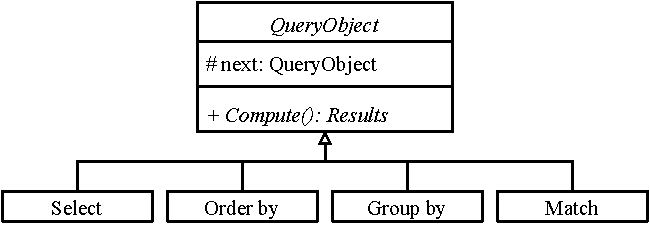
\includegraphics{../img/diaQueryObjects.pdf}\centering
\caption{UML class diagram objektů představující části dotazu.}
\label{figure.diaQueryObjects}
\end{figure}

\clearpage

\begin{figure}[!htp]
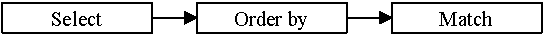
\includegraphics{../img/diaQueryObjectsCon.pdf}\centering
\caption{Propojení objektů pomocí položky \texttt{next} pro dotaz select x match (x) order by x.}
\label{figure.diaQueryObjectsCon}
\end{figure}

\begin{figure}[!htp]
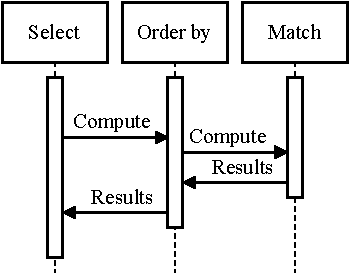
\includegraphics{../img/diaQueryObjectsCall.pdf}\centering
\caption{UML activity diagram rekurzivního volání metody \texttt{Compute} pro dotaz select x match (x) order by x.}
\label{figure.diaQueryObjectsCall}
\end{figure}

\subsection{Paralelizace vykonání dotazu}

Poslední věc nutnou ošetřit je způsob paralelizace dotazu.
Existuje několik možností.
Paralelizace bude provedena pouze interně pro každy objekt nebo dojde k vypracování složitějšího modelu.
V naší představě bychom volili první variantu.
Pomocí ní zaručíme nezávislost objektů a nebudeme nutni vytvářet závislosti mezi objekty.
Při analýze jednotlivých částí budeme vycházet z předpokladu, že existuje \texttt{ThreadPool} vláken.
Do \texttt{ThreadPool} budeme zařazovat úkony k vykonání (\texttt{Tasks}).

\subsection{Formát výsledků} \label{anal.tables}

Mezi částmi dochází k předávání výsledků.
Výsledky musí mít definovaný formát, aby každá část dokázala správně provádět svou logiku.
V části Match dochází ke generování obecných výsledků.
V části Group by dojde k vytvoření skupin a výpočtů agregačních funkcí.
Pokud je v uživatelském dotazu zahrnuto Group by, tak zbylé části musí očekávat jiný formát výsledků.
Daný formát musí obsahovat skupiny a výsledné hodnoty agregačních funkcí.

Obecné výsledky hledání budeme ukládat do tabulky.
Jeden řádek tabulky bude reprezentovat jeden výsledek hledání.
Nyní musíme rozhodnout, jaké informace do tabulky uložíme.
V části Match se pracuje s elementy grafu.
Jeden výsledek hledání obsahuje seznam elementů, které odpovídají vzoru.
Máme dvě možnosti, jak daný výsledek zpracovat.
První varianta v části Match při jeho nalezení vypočte hodnoty všech výrazů obsažených ve zbytku dotazu.
Sloupeček představuje hodnoty jednoho výrazu.
Tato varianta nám nepřišla vhodná, protože by objekt Match musel znát informace o výrazech v celém dotazu.
Navíc výrazy v částech mohou být rozdílné.
Tedy se vytváří nutnost vytvářet sloupečky hodnot v moment, kdy se nepotřebují a tím se navyšuje spotřeba paměti.

\clearpage

Příkladem může být dotaz: 
\begin{code}
select x.P1, ..., x.Pn match (x) -> (y) order by y.P1, ..., y.Pm  
n, m belongs to N and n, m > 1
\end{code}

Zde vidíme množství výrazů.
Pokud bychom aplikovali první variantu, tak v Match části musíme vygenerovat $m + n$ sloupců hodnot.
Z tohoto důvodu chceme zvolit jinou variantu.
Do tabulky budeme ukládat elementy grafu.
Sloupeček tabulky bude reprezentovat jednu proměnnou z dotazu Match.
Tedy tabulka má počet sloupečku rovný počtu unikátních proměnných. 
Pro stejný dotaz vytvoříme pouze dva sloupečky.
Abychom zamezili stejnému problému i z opačné strany (tj. mnoho proměnných a málo výrazů), tak budeme ukládat pouze proměnné, ke kterým se přistupuje v ostatních částech.
Tímto jsme vyřešili paměťový problém, ale nastal problém výkonnosti.
Vyvstává totiž nutnost vypočítávat hodnoty výrazů znova, přestože jsme je už v minulosti počítali (např. při třídění se několikrát porovnává stejný výsledek s jinými).
Problém se dá částečně řešit cachováním výsledků, ale ten ponecháme na analůzu zbylých částí.
V tento moment jsme se rozhodli jít cestou menší paměťové náročnosti na úkor výkonnosti.
Pro výsledky Group by můžeme opět v představě volit tabulku.
Jediný rozdíl bude, že řádek zde bude reprezentovat jednu skupinu (opět uložené elementy grafu) společně s vypočtenými hodnotami agregačních funkcí.

\subsection{Proxy třída jako řádek tabulky}

Musíme být schopni pracovat s řádky tabulek.
Pomocí řádků v tabulce se musí vyhodnotit výrazy v částech Group/Order by a Select.
Vstupním argumentem expression by měl být pouze jeden řádek.
Přesouvání řádku o více sloupcích je drahé.
Pro docílení efektivní práce s řádky budeme řádek reprezentovat proxy třídou.
Proxy třída bude návratová hodnota funkce indexeru tabulky (\texttt{ResultTable[i]}, kde \texttt{i} je index řádku).
Třída poskytne metody pro přístup k elementům nebo výsledkům agr. funkcí ve sloupečcích pro daný řádek tabulky.
V ideálním případě si bude pamatovat pouze index reprezentujícího řádku a odkaz na tabulku.
Nyní pokud budeme chtít vyhodnotit výraz pro $i$-tý řádek tabulky, tak zavoláním indexeru dostaneme proxy třídu a tu použijeme k vyhodnocení výrazu.

\bigskip
\textit{Analyzovali a navrhli jsme obecně způsob vykonání dotazu společně s formátem předávaných výsledků mezi částmi. 
Nyní přejdeme k analýze jednotlivých částí dotazu. 
V analýze jsme se rozhodli vychenat část Select, protože není podstatná pro naši práci.}

\section{Match a prohledávání grafu} \label{anal.match}

Match část má za úkol najít všechny podgrafy v grafu odpovídající zadanému vzoru.
Vlastnosti hledání jsou definované jazykem PGQL (sekce \ref{req.pgql}).
Vzor se vždy skládá z posloupnosti vrcholů a hran.
Na každý prvek posloupnosti se můžeme dívat jako na placeholder nějakého elementu grafu.

Vlastnosti hledání:
\begin{itemize}

\item Výsledky hledání jsou podgrafy homomorfní se zadaným vzorem.
\item Hrana se může opakovat několikrát v rámci jednoho vzoru.
\item Proměnná hrany ve vzoru se může použít pouze jednou.
\item Dvě rozdílné proměnné mohou obsahovat stejný element.
\item Shodnost elementů se ověřuje pouze na opakující se proměnné.

\end{itemize}

\subsection{BFS vs DFS}

Hledání podgrafu v grafu je obecně složitý problém. 
Cílem této práce není navrhnout algoritmus pro vyhledávání vzoru, proto jsme se rozhodli inspirovat a použít obecný postup k řešení daného problému.
Mezi základní postupy vyhledávání vzoru patří prohledávání do šířky (BFS) a prohledávání do hloubky (DFS) \citep[kap. 4]{graphAlg}. 
Na základě 1. a 2. kapitoly článku \citet{asyncPGX} jsme vybrali algoritmus DFS, jelikož v průběhu prohledávání generuje menší množství mezivýsledů.
To je dáno chováním BFS. 
BFS v každém kroku musí prozkoumat všechny sousedy políček z předešlého kroku.
Toho se docílí vložením nových sousedů do fronty (obecná struktura \texttt{queue} FIFO).
Fronta se tak rychle zvětšuje.
DFS naopak potřebuje znát sousedy pouze aktuálně prohledávaných vrcholů.

\subsection{Hledaný vzor a finální výsledek} \label{anal.match.res}

K aplikaci algoritmu musíme vytvořit strukturu (vzor) představující hledaný podgraf.
Strukturu budeme chápat jako propojené posloupnosti tříd.
Třída obsahuje informace specifikující vhodný element grafu, který ji má náležet.
Cílem DFS je nalézt elementy grafu, které budou odpovídat hledaným posloupnostem.
V průběhu DFS hledání si vzor pamatuje aktuální třídu, pro kterou DFS hledá vhodný element.
V moment průchodu DFS přes nějaký element se ověří zda se jedná o vhodný element pro aktuální třídu.
Pokud ano, třída nyní reprezentuje daný element, DFS z něj pokračuje v hledání a dojde k přestupu na další třídu v posloupnosti.
Pokud ne, DFS se vrací na předchozí element v hledání, ze kterého vybere následující element procházení.

\subsubsection{Tvorba vzoru}

Nyní musíme strukturu vytvořit.
V sekci \ref{anal.mathcandvar} jsme uvedli, že posloupnosti oddělené čárkou v Match části budou reprezentovány jako pole tříd obsahující informace o proměnných.
Tedy jedno pole je ekvivalentní jedné posloupnosti.
Pro zřetelnost budeme hovořit o jednom poli jako o řetězci.

Příklad dotazu se dvěma řetězci:
\begin{code}
match (x) -> (y), (x) -> (q)
\end{code}

Řetězce nám nyní budou sloužit k vytvoření vzoru.
Abychom mohli efektivně hledat daný vzor, potřebujeme z řetězců vytvořit souvislou komponentu.
Vytvoříme ji propojením řetězců pomocí opakujících se proměnných.
Tedy dva řetězce jsou propojeny právě tehdy, obsahují-li stejnou proměnnou. 
Propojením všech takových řetězců vytvoříme souvislou komponentu.
Souvislá komponenta představuje hledaný vzor.
Strukturu tedy chápeme jako abstrakci procházení DFS.
Problém vyvstane, pokud nám vzniknou dvě separátní komponenty z jednoho dotazu.
Tento případ nastene právě tehdy, když pro dvě komponenty neexistuje proměnná, která by je propojila.
V takovém případě se můžeme dívat na dotaz, jako na skalární součin výsledků hledání dvou komponent.
Stejný princip aplikujeme, pokud existuje vícero separátních komponent.

Příklad dotazu separátních komponent:
\begin{code}
select x, y match (x), (y)
\end{code}

\subsubsection{Finální výsledek}

Součástí struktury musí být také aktuální pole elementů představující proměnné dotazu (např. z výše uvedeného dotazu proměnné x a y).
Jedna položka v poli odpovídá jedné proměnné.
Bude existovat pouze jedno pole pro jeden vzor. 
Nebudou se vytvářet další, pouze se budou měnit obsahující elementy, protože chceme omezit režii za tvorbu polí.
Pole bude sloužit k ověření zda držíme totožné elementy v moment opakující se proměnné v průběhu hledání.
V moment nalezení celého podgrafu bude pole proměnných zaplněné a bude chápáno jako finální výsledek hledání, protože pouze proměnné jsou přístupné v jiných částech dotazu.

\subsection{Průběh hledání}

K nalezení všech podgrafů v grafu pořebujeme z každého vrcholu spustit DFS.
Při DFS se bude kontrolovat, jestli průchod odpovídá hledanému vzoru.
Procházení vždy začíná vrcholem, následně přístupem k hranám daného vrcholu a pak koncovému vrcholu hrany. 
K procházení grafu máme navrhnutou strukturu z sekce reprezentace grafu \ref{anal.grafrep}.
Pokud dojde k nalezení podgrafu, tak výsledek bude uložen způsobem z sekce \ref{anal.tables}.
V našem případě tedy překopírování elementů z pole proměnných náležící vzoru.

Vyhledávání separátních komponent vyřešíme následovně.
V momentě, kdy nalezneme podgraf odpovídající jedné komponentě, tak se spustí DFS vyhledávání pro komponentu další.
Teprve až projdeme všechny komponenty, výsledek se uloží do tabulky.
V tuto chvíli budeme vlastnit finální výsledek hledání, který můžeme uložit do tabulky.
Zbavíme se tak nutnosti uchovávat mezivýsledky a následnému tvoření skalárního součinu.

\subsection{Paralelizace hledání} \label{anal.matchPar}

Nyní přistoupíme k analýze paralelizace hledání.
V paralelním řešení chceme použít co nejmenší počet synchronizačních primitiv.
Ukládání výsledků do společné struktury by způsobilo značnou režii za synchronizaci.
V ideálním případě bude probíhat hledání lokálně, následně pak dojde k efektivnímu slévání výsledků.

Jako řešení jsme zvolili jeden ze základních způsobů.
Budeme paralelizovat prohledávání ze startovních vrcholů.
Vyhledávání bude reprezentováno objektem (\texttt{Matcher}).
\texttt{Matcher} vlastní strukturu reprezentující hledaný vzor (\texttt{Pattern}).
Každé vlákno bude vlastnit lokálně svůj \texttt{Matcher}, \texttt{Pattern} a svou tabulku výsledků.
Všechna vlákna budou sdílet thread-safe objekt, který přiděluje části vrcholů grafu (\texttt{VertexDistributor}).
Vlákno vždy zažádá \texttt{VertexDistributor} o určitý počet vrcholů, ze kterých spustí lokálně prohledávání a výsledky uloží do své tabulky.
Nikdy nenastave situace, kdy dva vlákna mají stejný startovní vrchol.
Po vyčerpání všech vrcholů grafu prohledávání končí.
V jednovláknovém řešení jsou přiděleny všechny vrcholy najednou danému vláknu. 
Rozložení objektů mezi vlákny je zobrazeno na obrázku \ref{figure.diaQueryObjectsMatchPar}. 

\texttt{VertexDistributor} je zde velice důležitý.
Musí rozdělovat malé části vrcholů.
Kdyby rozděloval velké části vrcholů může se stát, že některá vlákna budou mít mnohem více práce.
Je to protože reálné grafy nemají obecně rovnoměrné rozložení hran.
Jedno vlákno by mohlo dostat vrholy nacházející se v oblasti s množstvím hran, zatímco jiné vlákno by procházelo řídkou oblastí.
Jelikož se rychle vyčerpaly startovní vrcholy, tak vlákno z řídké oblasti ukončí svou práci mnohem dříve něž vlákno první.
Nyní se musí čekat na dokončení práce prvního vlákna.

\subsection{Slévání výsledků hledání}

Po dokončení hledání je nutno vyřešit slévání výsledků jednotlivých vláken.
Kdybychom ponechali výsledky bez úpravy, tak nedokážeme rovnoměrně rozdělit práci mezi vlákna v paralelních řešeních Order/Group by.
Cílem je vytvořit jednu tabulku obsahující všechny výsledky.
K vyhnutí překopírovávání všech výsledků vláken využijeme následující princip.
Sloupeček tabulky bude tvořen polem polí fixní délky.
V jazyce C\# \texttt{List<Element[FixedArraySize]>}.
V kroku slévání nyní pouze překopírujeme odkazy na pole místo samotných výsledků.
Avšak, pořád nám zůstává nutnost překopírovat výsledky posledních polí sloupečků, která jsou nezaplněná.
Volbou vhodné hodnoty \texttt{FixedArraySize} se bude překopírovávat pouze malé množství výsledků.
Konkrétní volba hodnoty je heuristická a vyplývá z vlastností grafu a počtu nalezených výsledků.
Pro naše učely během implementace zkusíme zvolit prvně $n/\log_2 n$ ($n = $ \#výsledků hledání) pro jednovláknové a pro paralelní zpracování $(n/\log_2 n)/\#threads$.
$log_2 n$ odpovídá počtu přealokování při plnění dynamického pole $n$ položkami.
Slévání bude probíhat opět paralelně.
Nabízí se dva způsoby.
Vlákno slévá pouze jeden sloupeček nebo dojde k dvoucestnému slévání výsledků vláken.
Nyní je obtížné odhadnou správné řešení a proto jej ponecháme na dobu implementace.    

\clearpage

\begin{figure}[!htp]
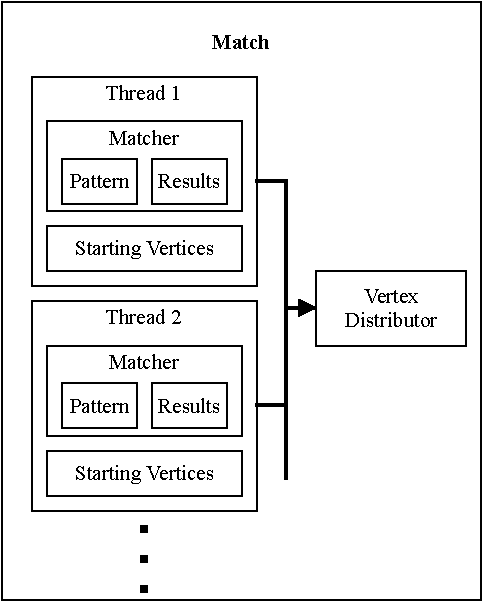
\includegraphics{../img/diaQueryObjectsMatchPar.pdf}\centering
\caption{Diagram paralelizace prohledávání grafu.}
\label{figure.diaQueryObjectsMatchPar}
\end{figure}

\bigskip
\textit{Zbývá nám analyzovat a navrhnout Group by a Order by.
Je nutné si uvědomit potřebu analýzy daných částí.
Analýza nám pomůže pochopit jejich fungování, což nám umožní je lépe porovnat s vylepšenými řešeními. 
Zároveň také tvoří odrazový můstek pro návrh vylepšených řešení.}


\section{Order by}

Order by si klade za cíl setřídit vyhledané výsledky z části Match pomocí zadaných klíčů.
Pořadí klíčů určuje pořadí porovnání.
Výsledky se porovnávají zleva doprava.
To znamená, pokud jsou dva klíče stejné, postoupí se k porovnání s klíčem dalším.
Rovnost dvou výsledků nastává právě tehdy, když mají stejné hodnoty pro všechny klíče. 
Pro klíč se také definuje, jestli má třídění probíhat v rostoucím nebo klesajícím pořadí.
Defaultní pořadí je chápáno jako rostoucí. 
Potřebujeme určit, jakým způsobem budou výsledky hledání setříděny.
Musíme vybrat algoritmus a následně navrhnout způsob efektivního třídění tabulky výsledků.

\subsection{Výběr algoritmů a paralelizace}

Existuje mnoho algoritmů pro třídění.
Chtěli bychom zvolit již prozkoumané a zároveň běžně používané třídící algoritmy.
Mezi náš výběr padli Merge sort nebo Quick sort.
Jsou ideální volba, protože pro ně již existuje paralelní verze.
Při implementaci chceme ideálně použít již existující knihovny nebo implementace. 

\subsection{Quick sort vs Merge sort}

Uvedeme krátké porovnání na základě 3. kapitoly průvodce algoritmů \citep{labyrint}. 
Merge sort má časovou složitost $ \Theta(n\log n) $ i v nejhorším případě, zatímco Quick sort stejné složitosti dociluje pouze v průměrném případě.
V nejhorším případě má $\Theta(n^2)$.
Merge sort potřebuje $\Theta(n)$ pomocné paměti a je to stabilní třídící algoritmus.
Quick sort pouze $\Theta(\log n)$, ale nejedná se stabilní třídění.
K implementaci stabilního Quick sortu je potřeba $\Theta(n)$ pomocné paměti.
Quick sort značně závisí na výběru pivota.
V našem případě bude obtížné ho volit správně, protože nedokážeme říci nic o rozložení tříděných dat.
Z tohoto důvodu bychom volili raději Merge sort.  

\subsection{Třídění pomocí indexů}

Hlavním problémem Order by je třídění tabulky výsledků.
V sekci \ref{anal.tables} jsme definovali formát výsledků a navrhli proxy třídy pro výpočet výrazů.
Setřídit tabulku v našem smyslu znamená setřídit řádky pomocí klíčů zadaných uživatelem.
Pro zjištění shodnosti dvou řádků musíme vypočítat hodnoty jejich klíčů pomocí výrazů a následně je porovnat.
Přesouvání řádků v tabulce, která má více než jeden sloupec, by představovalo značné zpomalení.
Uvedli jsme, že výrazy pro řádky dostanou na vstupu proxy třídu řádků.
Proxy třída se v naší představě získá voláním funkce indexeru na tabulce výsledků.
Daný princip nám umožní vytvořit pole indexů v rozsahu počtu řádek tabulky.
Indexy budou setříděny namísto pravých řádků vybraným algoritmem a při porovnání dojde k získání proxy tříd a výpočtu výrazů.
Přistup nám umožní vyřadit přesouvání řádků, ale zase potřebujeme lineární pamět na pole indexů.
Po dokončení třídění se pole použije jako indexační struktura.

\subsection{Optimalizace porovnání vlastností hodnot} \label{anal.order.opt1}

Třídění obvykle představuje opakované porovnání jednoho prvku s ostatními v řadě za sebou.
Pro pokaždé takové porovnání v řadě počítáme stejnou hodnotu výrazu opakovaně.
Porovnání pomocí \texttt{ID} pouze přistupuje k položce elementu grafu.
Problém nastane, když budeme porovnávat pomocí vlasnosti.
V takovém případě musíme přistoupit k tabulce \texttt{elType} (sekce \ref{anal.grafrep}), zjistit existenci přistupované vlastnosti a následně přistoupit k její hodnotě.
Danou situaci můžeme vyřešit částečně cachování výsledků výrazů.
Budeme si pamatovat poslední porovnané řádky a jejich hodnoty.
Pokud dojde k porovnání řádků pro který byl výraz již vypočítán, tak použijeme zachovanou hodnotu.

\subsection{Optimalizace porovnání stejných elementů}

Dalši možná optimalizace porovnání může nastat v případě, pokud pro použitý graf platí \#Vrcholů $<<$ \#Hran.
Daná vlastnost může mít za následek, že porovnávané řádky budou často obsahovat stejné elementy pro dotazy typu:
\begin{code}
select x.PropOne match (x) -> (y) order by x.PropOne;
\end{code}
V takovém dotazu by hledání mělo vygenerovat několik výsledků se stejným elementem v proměnné x.
Počet takových výsledků zde odpovídá počtu hran vrcholů x.
Abychom předešli opakovanému porovnávání hodnot vlastností stejných elementů, tak než přistoupíme k výpočtu výrazů porovnáme \texttt{ID} přistupovaných elementů.
Tedy využijeme dvou optimalizací.
Budeme si cachovat poslední výsledky výrazů a navíc omezíme porovnání výsledků se stejnými elementy.

\subsection{Optimalizace v paralelním prostření}

Vymysleli jsme optimalizace porovnání.
Doteď jsme však předpokládali, že porovnání probíhá v jednom vlákně.
Druhá optimalizace funguje i v paralelním prostřední, protože se jedná pouze o čtení statických hodnot.
Avšak první optimalizace vytváří problém.
V prvním případě dochází k uchovávání výsledků lokálních pro vlákno a existence sdíleného úložiště by vytvořilo souběh.
Vlákna by se snažila číst a ukládat výsledky ze sdíleného úložiště a docházelo by k nedefinovanému chování.
Problém se dá vyřešit například tak, že každé vlákno bude vlastnit svoje objekty s cachí výsledků.
V průběhu implementace budeme muset najít vhodnou techniku ukládání, aby došlo ke zrychlení třídění.

\section{Group by}

Group by seskupuje výsledky hledání podle uživatelem zadaných klíčů.
Dva výslekdy patří do stejné skupiny právě tehdy, když se shodují ve všech hodnotách klíčů.
Musíme být schopni vypočítat agregační funkce pro skupiny.
K tomu již máme navržené způsoby z sekce Expressions (\ref{anal.expressions}).
Zbývá nám vymyslet způsob ukládání mezivýsledku a algoritmy k vykonání.

\subsection{Módy Group by}

Group by představuje dle našeho pohledu dva módy vykonání.
První mód obsahuje v dotazu část Group by a libovolné množství agregačních funkcí.
Dojde k vytvoření skupin a výpočtu výsledků funkcí pro každou skupinu.
Tento mód budeme označovat \textbf{Group by}.
Druhý mód nemá v dotazu část Group by, ale pouze agregační funkce v ostatních částech.
Zde automaticky dochází k předpokladu, že všechny výsledky patří do stejné skupiny.
Tedy je vytvořena pouze jedna skupina a pro ni se vypočtou hodnoty agregačních funkcí.
Mód nazveme \textbf{Single group Group by}.


\subsection{Úložiště mezivýsledků agregačních funkcí} \label{anal.groupby.uloziste}

V sekci Expressions (\ref{anal.expressions}) jsme navrhli objekt, který obsahuje logiku výpočtu funkce a na vstupu dostává úložiště výsledku.
Očekává se, že pro každou skupinu bude existovat úložiště.
Úložiště musí obsahovat prostor pro výsledky všech počítaných funkcí.
Vymysleli jsme dva způsoby:

\begin{itemize}

\item \textbf{Bucket} - každá skupina bude vlastnit pole objektů. 
Pole bude mít délku rovnou počtu počítaných agregačních funkcí.
Objekty představují úložiště výsledků funkcí.

\item \textbf{List} - výsledky všech skupin jsou uchovávány v dvoudimenzionálním poli, tj. primitivní tabulce.
Sloupeček představuje výsledky jedné agregační funkce.
Jedné skupině pak přináleží řádek.
Každé skipině bude přidělen index řádku.
Nyní pokud budeme chtít výsledky funkcí skupiny, stačí přistoupit skrze přidělený index ke chtěnému výsledku.
\end{itemize}

Následuje ukázka možné implementace dle popisu výše v jazyce C\#:
\begin{code}
Bucket:
\\ Pole výsledků ag. funkcí.
BucketResult[] groupAggFuncResults; 
\\ Objekt úložiště. 
class BucketResult {} 
\\ Objekt definující typ ukládané hodnoty.
class BucketResult<T>: BucketResult { T value; }

List:
ListResults groupsAggFuncResults;
\\ Objekt primitivní tabulky výsledků ag. funkcí.
class ListResults { ListHolder[] holders; }
\\ Objekt jednoho sloupečku tabulky.
class ListHolder {}
\\ Objekt definující typ sloupečku.
class ListHolder<T> : ListHolder { List<T> values }
\end{code}

První způsob je náročnější na paměť oproti druhému způsobu, neboť je zde nutnost vytvářet objekty a pole pro každou skipinu.
Avšak, v druhém způsobu jsme nuceni přistupovat k výsledkům pomocí indirekce.
Výhoda Bucket spočívá v jeho jednoduchém přemisťování (chápeme-li pole jako referenci) a izolaci od ostatních výsledků skupin.
V takovém případě jsme schopni přesouvat výsledky skupiny aniž bychom museli kopírovat jejich hodnoty.
Předpokládáme, že bucket bude výhodnější pro paralelní zpracování díky izolaci od ostatních výsledků, jelikož počet skupin není dopředu znám.
V List budeme muset dynamicky rozšiřovat pole.
Při rozšíření nastane souběh, který budeme muset ošetřit.

\subsection{Logika agregačních funkcí}

Ještě než přistoupíme k výběru zpracování musíme analyzovat logiku agregačních funkcí.
Logika pak ovlivňuje co a jak se bude ukládat v úložišti výsledků.

\begin{itemize}
\item \texttt{Min/Max:} výsledek funkce je minimum/maximum pro skupinu. Při výpočtu dojde k porovnání a následnému uložení hodnoty.
V objektu výsledku musíme znát aktuální minimum/maximum.
Dále, byla-li hodnota již nastavena, protože musíme být schopni rozeznat prázdné úložiště po jeho vytvoření.


\item \texttt{Count/Sum:} výsledek je počet výsledků/suma hodnot výsledků. Při výpočtu musíme přičítat hodnotu k hodnotě v úložišti.
\item \texttt{Avg:} výsledek je aritmetický průměr. Chtěli bychom volit inkrementální metodu. Budeme si ukládat počet výsledků a sumu hodnot výsledků. Pro získání finální hodnoty dojde k vypočtení podílu sumy a počtu výsledků.
\end{itemize}

\subsection{Jednovláknové zpracování}

Po celou dobude budeme pracovat s tabulkou výsledků Match části.
Pro vykonání Group by se nám nabízí několik možností.
První možnost je řádky tabulky setřídit a následně při iteraci výtvářet skupiny a počítat agregační funkce.
Myslíme, že možnost přináší zbytečnou režii za porovnání při třídění, protože pro každé porovnání musíme vypočítat hodnotu výrazu.
Z tohoto důvodu chceme využít strukturu, která bude interně použivát hašovací tabulku (C++ \texttt{std::map<Key, Value>} nebo C\#  \texttt{Dictionary<Key, Value>}).
Záznam v tabulce bude dvojice \texttt{key/value}. 
\texttt{key} je zde index do tabulky výsledků z Match části (nikoliv proxy třída).
Chceme ukládat pouze index abychom ušetřili paměť za pointr na tabulku.
Porovnání vyvolá získání proxy třídy a následné evaluaci hodnot výrazů.
\texttt{value} obsahuje strukturu pro výsledky agregačních funkcí.
Pro Bucket to bude pole objektů a pro List to bude index do tabulky výsledků agregačních funkcí.
Pro výsledek bude vypočítáná haš na základě hodnot klíču a vložena do hašovací tabulky.
Pokud už je obsažen v tabulce, tak se pouze pro získanou \texttt{value} (pole nebo index) aktualizují hodnoty výsledků agregačních funkcí.
V opačném případě bude vložen nový záznam s novou \texttt{value}.
Pro Single group Group by stačí pouze iterovat skrze tabulku a počítat agregační funkce.

\subsection{Optimalizace při výpočtu haš hodnoty}

Minulý přístup nám nabízí jednu optimalizaci k ušetření opakovaného výpočtu hodnoty výrazu klíčů.
Hašovací tabulka při vložení dvojice v prvním kroku vypočte hodnoty klíčů a vypočte jejich haš.
Výsledek se vloží do patřičné přihrádky.
Pokud nastala kolize, tak se prvky musí porovnat.
Při tomto porovnání se opět musí vypočíst hodnoty výrazů vkládané dvojice.
Zde mužeme využít chvíle výpočtu haš hodnoty.
Budeme cachovat hodnoty výrazů a následně je znovu použít při porovnání.
Nicméně, pravděpodobně budeme nutni vytvořit závislost mezi objektem počítajícím haš hodnotu a objektem provádějícím porovnání.
Stejný princip jsme použili při optimalizaci porovnání v sekci \ref{anal.order.opt1}.
Nastávají pro něj také stejné problémy v paralelním prostředí.

\subsection{Paralelní zpracování}

Chceme zvolit několik řešení s rozdílnou úrovní synchronizace, protože nevíme, které bude dosahovat nejrychlejších výsledků.
Navíc nám větší počet řešení umožní lépe porovnat vylepšená řešení.
Pro paralelní zpracování jsme vymysleli tři přístupy: \textbf{Global}, \textbf{Two-step} a \textbf{Local + dvoucestné slévání} (všechny budou schopny pracovat s úložišti Bucket i List).
Každý z nich začíná rozdělením tabulky výsledků Match na ekvivalentní části.
To si můžeme dovolit, neboť máme tabulku obsahující všechny výsledky hledání.
Každé vlákno dostane danou část ke zpracování.
Tím zaručíme rovnoměrnost práce mezi vlákny.
Samotná práce vláken pak zavisí na zvoleném přístupu.
Specifika vykonání jsou popsána v následujících sekcích.

\subsection{Thread-safe agregační funkce}

Ještě než přistoupíme k popisu jednotlivých řešení, je důležité si uvědomit nutnost vytvořit thread-safe verzi objektů implementující logiku agregačních funkcí.
Pro každou funkci bude existovat ekvivalent thread-safe \texttt{Apply} metody.
Samotně pak vyvstává nutnost implementovat thread-safe metody pro slévání výsledků agregačních funkcí.
Problém vyřešeníme přidáním metod do objektů zpravující logiku agregačních funkcí, protože při slévání stále musíme vědět, jak s výsledky správně zacházet.
Pro úpravu logiky agr. funkcí na thread-safe verze volíme tyto varianty:

\begin{itemize}

\item \texttt{Min/Max:} princip Compare and Exchange. V moment porovnání mohlo dojít ke změně hodnoty v úložišti.
Musíme znovu provést porovnání.  

\item \texttt{Sum/Count:} tyto metody implementují pouze přičítání. 
V ideálním případě chceme použít atomické operace přičtění.
 
\item \texttt{Avg:} tuto funkci lze implementovat iterativně. 
Budeme si ukládat součet zpracovaných výsledků a jejich počet.
Finální hodnota pak bude podíl součtu a počtu hodnot.
Tímto můžeme implementovat thread-safe funkci pomocí atomických operací, jako u funkcí \texttt{Sum/Count}.
\end{itemize}

\subsection{Global Group by} \label{anal.groupby.global}

Všechna vlákna budou provádět ekvivalent jednovláknového zpracování pomocí thread-safe paralelní mapy/slovníku (C\# \texttt{ConcurrentDictionary, Java \texttt{ConcurrentHashMap}}).
Skupiny se vytváření globálně.
Všimněme si nutnosti dvojité synchronizace.
Prvě musí dojít k synchronizaci vytváření záznamů v mapě.
Druhý krok synchronizace je nutný při zpracování agregačních funkcí.
Paralelní mapa nám vyřadí souběh při vytváření nových záznamů skupin.
V moment zpracování agregačních funkcí musí dojít k volání thread-safe verzí.
Výhoda této metody je, že nedochází ke slévání, tj. po dokončení práce vlákny jsou výsledky finální.

Bucket reprezentace úložiště má zde značnou výhodu vůči List.
List musí dynamicky rozšiřovat tabulku svých výsledků.
Místo abychom použili dvojí synchronizace jako u Bucket, tak zde bude nutné představit ještě třetí krok synchronizace.
Při přístupu do tabulky je nutné kontrolovat, jestli se nemusí rozšířit.
V ten moment se musí zabránit přístupu ostatních vláken a teprve pak rozšířit tabulku.
To se dá implementovat například semaforem omezující pohyb vláken v kritické sekci.
Vlákno v moment nutnosti rozšíření zablokuje vstup přes semafor.
Vlákno se na přístup pokusí projít skrze semafor, pokud je mu vstup zabráněn tak dochází k rozšiřování tabulky.
V opačném případě aktualizuje výslednou hodnotu agregační funkce.
Postup s List může být však značně pomalý a proto budeme uvažovat, jestli přístup raději implementovat pouze pro Bucket.
Global Group by je znázorněn na obrázku \ref{figure.diaGlobalGr}.

\subsection{Two-step Group by} \label{anal.groupby.twostep}

Tento přístup probíhá ve dvou krocích.
Lokální část nasledovaná globální částí. 
V lokální části pro každé vlákno běží kompletně identický ekvivalent jednovláknového zpracování.
Globální část nastane v moment dokončení této práce.
Místo aby vlákno ukončilo běh, tak rovnou provede slévání svých výsledků do thread-safe paralelní mapy.
To znamená, že vlákno nečeká na dokončení práce ostatních vláken, ale rovnou slévá své výsledky do paralelní mapy.
Tento přístup kombinuje jednovláknové řešení společně s přístupem Global.
Mínus je, že zde musí docházet ke slévání, ale v prvním kroku se využívají metody, které nemusí řešit synchoronizaci. 
Problematická část je zde slévání výsledků s List úložištěm výsledků agregačních funkcí.
První fáze nepředstavuje problém. 
Druhá představuje problém jako u Global řešení, tedy platí vše, co jsme pro něj zmínili.
Můžeme zkusit implementovat stejné řešení jako u Global pomocí semaforu.
Two-step Group by je znázorněn na obrázku \ref{figure.diaTwoGr}.

\subsection{Local + dvoucestné slévání Group by} \label{anal.groupby.local}

Přístup nepoužívá thread-safe metody ani paralelní mapu.
Opět rozdělíme přístup na dvě části.
V prvník kroku pro každé vlákno běží identický ekvivalent jednovláknového zpracování.
Po dokončení se spustí dvoucestný slévání na výsledky vláken.
Slévání bude připomínat binární strom.
Listy představují lokální seskupování vláken.
Vnitřní vrcholy stromu představují slévání výsledků.
Finální výsledek je vytvořen v kořeni.
U slévání využijeme paralelního zpracování.
Při slévání vždy jedno vlákno ukončí běh, druhé z dvojice provede slévání a postoupí ke kořeni. 
Hlavní výhody byly už zmíněny.
Používají se metody bez synchronizace.
Nevýhoda řešení je, že vlákna musejí čekat při slévání na dokončení práce druhého vlákna a teprve až pak může dojít ke slévání.
Přístup je znázorněn na obrázku \ref{figure.diaLocalGr}.

\subsection{Paralelizace Single group Group by}

K paralelizaci Single group Group by se nám poskytuje využít jíž zmíněných principů.
Konkrétně zde mají využítí všechny tři.
Slévání všech výsledků do jednoho úložiště výsledků agregačních funkcí z principu Global.
Problémem tohoto přístupu je synchronizace mnoha vláken na jednom místě.
Ideálnější je využít lokálního zpracování zbylých dvou metod.
Opět řešení rozdělíme na dva kroky. 
V prvním kroku každé vlákno provádí ekvivalent jednovláknového zpracování bez vytváření skupin, tj. počítá pouze agregační funkce pro jednu skupinu.
Výsledky se následně musí slévat.
K rozhodnutí, které řešení finálně použít použijeme fakt, že počet výsledků k slévání je roven počtu vláken.
V takovém případě nebudeme implementovat paralelní slévání, ale pouze jedno vybrané vlákno provede sjednocení všech výsledků.


\begin{figure}[!htp]
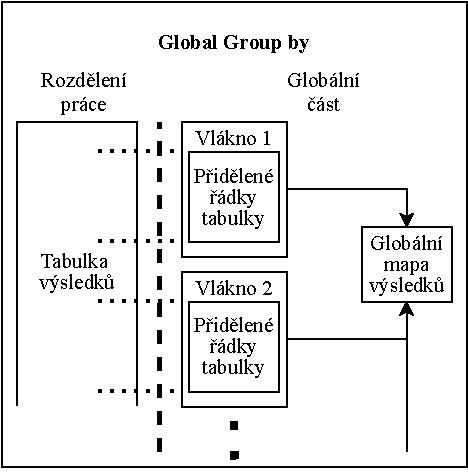
\includegraphics{../img/diaGlobalGr.pdf}\centering
\caption{Diagram paralelizace Global Group by.}
\label{figure.diaGlobalGr}
\end{figure}

\begin{figure}[!htp]
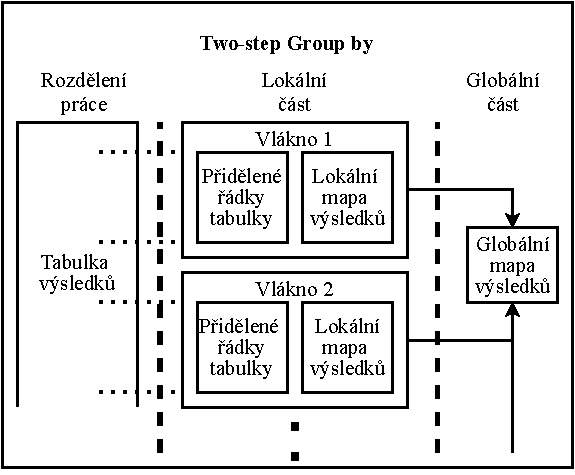
\includegraphics{../img/diaTwoGr.pdf}\centering
\caption{Diagram paralelizace Two-step Group by.}
\label{figure.diaTwoGr}
\end{figure}

\clearpage

\begin{figure}[!htp]
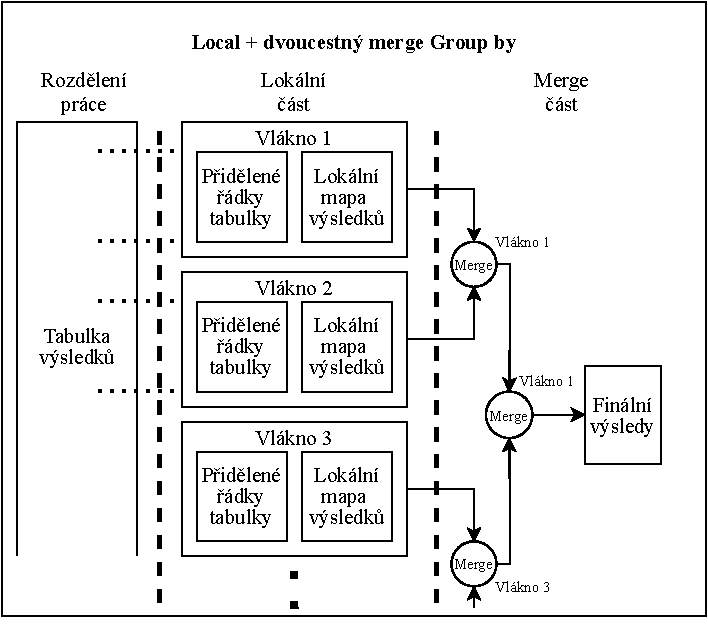
\includegraphics{../img/diaLocalGr.pdf}\centering
\caption{Diagram paralelizace Local + dvoucestné slévání Group by pro 4 vlákna.}
\label{figure.diaLocalGr}
\end{figure}

\bigskip
\textit{Analyzovali jsme a navrhli řešení vykonání částí Match, Group by a Order by.
Tímto jsme dokončili analýzu a návrh dotazovacího enginu.
Daná analýza a návrh nám poskytnou odrazový můstek při analýze úprav pro vykonání částí Group by a Order by v průběhu hledání.
}
%%%%%%%%%%%%%%%%%%%%%%%%%%%%%%%%%%%%%%%%%%%%%%%%%%%%%%%%%%%%%%

\section{Úprava enginu} \label{anal.improvement}

Cílem úprav je poskytnout enginu schopnost provádět části Group by a Order by v průběhu prohledávání grafu části Match.
Obecně to znamená, že v moment nalezení jednoho výsledku jej musíme okamžitě zpracovat.
Pro Order by to znamená výsledek správně zatřídit do již setříděné posloupnosti výsledků.
Pro Group by to znamená výsledek přidat do správné skupiny nebo pro něj skupinu vytvořit, navíc musíme pro něj zpracovat agregační funkce. 
Čili, výsledky v průběhu hledání Match části nebudeme ukládat do tabulky, která se po nalezení všech výsledků předá k dalšímu zpracování.
Namísto toho navrhneme postup, kterým docílíme zpracování výsledků v moment jeho nalezení.
Postupy ověříme vůči stávajícím řešením v kapitole Experiment \ref{expr} z hlediska doby vykonání.
V ideálním případě docílíme zrychlení nebo pouze vyrovnání vůči řešením vykonávající Order by a Group by po dokončení hledání.
Z hlediska implementace to také znamená naprogramovat vylepšení tak, abychom byli schopni jednoduše přepínat mezi způsobem vykonání dotazu.
Řešení tedy musí fungovat nezávisle na sobě. 
V prvním kroku úprav musíme získat obecný pohled na pozměněný způsob vykonání dotazu.
Následně v dalších krocích budeme navrhovat části dotazu konkrétněji.

\subsection{Pohled na pozměněný způsob vykonání dotazu}

V následujicích sekcích popíše náš obecný pohled na zpracování dotazu.
Budeme vycházet z sekce \ref{anal.vykonanidotazu}.
V dané sekci jsme si definovali prioritu částí dotazu.
Priorita určovala pořadí vykonání:
\begin{code}
Match > Where > Group by > Having > Order by > Select
\end{code}
Match se provedl jako první.
Následně se nalezené výsledky předávali dalším částem ve směru klesající priority.
Nejvyšší priorita se nachází nalevo a nejnižší napravo.
Pro naše potřeby úprav budeme nyní uvažovat pouze části Match, Group by, Order by a Select.
Opět budeme o částech uvažovat jako o separátních objektech.
Potřebujeme, aby Match část v moment nalezení výsledku jej předala k zatřídění části Order by nebo k seskupení části Group by.
Po zatřídění/seskupení se opět pokračuje v prohledávání grafu, dokud se nenajde další výsledek a ten se zase předá k dalšímu zpracování.
Můžeme si všimnout značné podobnosti s předchozím návrhem. 
Jediný rozdíl je ten, že místo předání všech výsledku najednou další části se předá výsledek pouze jeden.
Na Match část se můžeme dívat jako na kontinuální generátor výsledků. 
V momentě nalezení se výsledek pošle dálším částem.
Zbylé části pak pouze čekají na moment příchozího výsledku.
Finální výsledky budou uchovány v objektech částí Group by nebo Order by. 

Otázkou je, co je zde předávaný výsledek.
Budeme předpokládat, že předávaný výsledek ke zpracování je pole promenných definové v sekci hledaného vzoru \ref{anal.match.res}.
To znamená, že předané pole se nesmí měnit, protože pole náleží struktuře vzoru.
Tedy pokud s ním chceme pracovat přímo, musíme vytvořit kopii.
\textbf{Když budeme hovořit o výsledku hledání, tak máme na mysli dané pole proměnných.}

\subsection{Order/Group by část jako bariéra}

Problematická sekce návrhu je část Select.
Pokud dotaz neobsahuje další části, pak v době nalezení výsledku jej stačí pouze vypsat.
Nicméně, pokud je v dotazu obsažen Group by nebo Order by, pak se výsledky mohou vypsat až po dokončení třídění nebo seskupování.
Tedy dané dvě části nám tvoří bariéru, skrze kterou nemůže posílat výsledky dále.
Jelikož máme navrhnout pouze vykonání částí Order by a Group by, tak budeme uvažovat pro Match a Select stejný návrh, jako v minulých sekcích.
Tedy dotaz bude tvořen původní částí Select propojenou s části Match.
Část Match pak propojíme s částmi Order/Group by a upravíme tak, aby jim byla schopna předávat jeden výsledek v moment jeho nalezení.  

\subsection{Změna objektů reprezentující části Order/Group by}

Řekli jsme, že budeme opět považovat části dotazu za separátní objekty.
Vytvoříme nové objekty částí Group/Order by reprezentující nový způsob zpracování.
Abychom byli schopni pracovat souběžně i s původními objekty, tak potřebujeme upravit objekt Match, protože musí chápat nový způsob zpracování. 
Reprezentanty částí Order by a Group by budou nyní nové objekty (obrázek \ref{figure.diaStreamedResultProcessor}).
Budou si implementovat logiku zpracování jednoho výsledku v metodě \texttt{ProcessResult}.
Objekt zároveň obsahuje finální výsledky dotazu, proto potřebujeme metodu \texttt{RetrieveResults} na jejich získání.

Dotaz bude reprezentován opět řetězcem jako před úpravou zpracování.
Select a Match budou tvořit propojení objetků na základě UML diagramů \ref{figure.diaQueryObjects} a \ref{figure.diaQueryObjectsCon}.
Propojení objektu Match s novými objekty Group by a Order by navrhneme v dalších částech.

\begin{figure}[!htp]
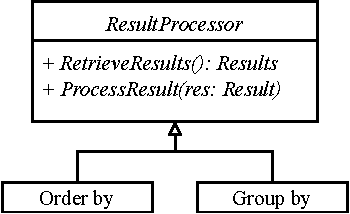
\includegraphics{../img/diaStreamedResultProcessor.pdf}\centering
\caption{UML class diagram nových objektů reprezentující části Group by a Order by.}
\label{figure.diaStreamedResultProcessor}
\end{figure}

\subsection{Propojení nových objektů s objektem Match}

Vytvořili jsme nové objekty a nyní je musíme propojit s objektem Match.
Objekty budou propojeny na dvou úrovních.
První úroveň bude přímé spojení nových objektů s objektem Match a druhá úroveň bude propojení vyhledávání a zpracování výsledku.

\subsubsection{Přímé spojení objektů}

Popíšeme realizaci první úrovně propojení, tj. objekt Match drží odkaz na objekt Group/Order by.
Abychom realizovali tuto úroveň, tak musíme upravit objekt Match.
Objekt Match rozšíříme o chápání logiky nových objektů (obrázek \ref{figure.diaStreamedQueryObjects}).
Stávající objekt Match jsme v naši představě pouze rozšířili a nevytvářeli kompletně nový objekt, protože propojení s Select objektem je realizováno stále původním způsobem.
Finální propojení objektů je pak znázorněno na obrázku \ref{figure.diaStreamedQueryObjectsCon}.

\begin{figure}[!htp]
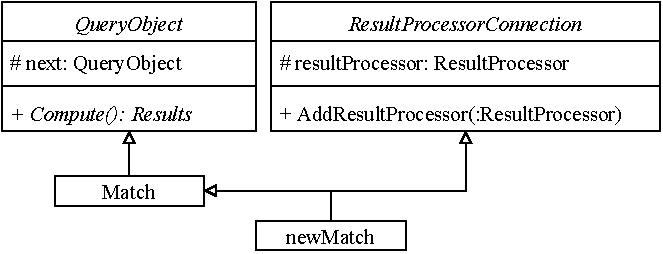
\includegraphics{../img/diaStreamedQueryObjects.pdf}\centering
\caption{UML class diagram rozšířeného objektu Match. Objekt nyní drží přímý odkaz na \texttt{ResultProcessor} a zároveň implementuje původní logiku objektu.}
\label{figure.diaStreamedQueryObjects}
\end{figure}

\begin{figure}[!htp]
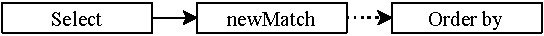
\includegraphics{../img/diaStreamedQueryObjectsCon.pdf}\centering
\caption{Diagram objektů upraveného vykonání představující části dotazu select x match (x) order by x. Plná šipka znázorňuje původní propojení a tečkovaná šipka představuje nové nové propojení.}
\label{figure.diaStreamedQueryObjectsCon}
\end{figure}


\subsubsection{Propojení vyhledávání a zpracování výsledku}

Musíme ještě navrhnout způsob předávání výsledků částem Order/Group by v průběhu hledání.
Způsob musí být použitelný pro paralelní zpracování, proto budeme rovnou přemýšlet nad paralelním řešením.
V naši představě budeme vycházet přímo z původního návrhu z sekce \ref{anal.match}.
Definovali jsme si, že každé vlákno vlastní lokálně strukturu vzoru \texttt{Pattern}, objekt vyhledávání \texttt{Matcher} a tabulku výsledků.
Finální výsledky ukládá do tabulky a po dokončení hledání dojde k slévání tabulek.
Zde upravíme část, kdy dochází k ukládání výsledků do tabulky.
Vlákno bude držet odkaz na objekt Group/Order by a v moment nalezení výsledek předá pomocí volání metody \texttt{ProcessResult}.
Metoda výsledek zpracuje a po návratu z metody se pokračuje ve vyhledávání.
To se opakuje dokud prohledávání neskončí.

Zpracování dotazu bude finálně vypadat následovně.
Na řetězci objektů se zavolá metoda \texttt{Compute}.
První objekt v řetězci je Select.
Select rekurzivně zavolá metodu na části Match a ta spustí vyhledávání.
Část Match prohledává graf a výsledky předává části Order/Group by pomocí metody \texttt{ProcessResult}.
Po dokončení prohledávání volaná metoda \texttt{Compute} na objektu Match získá zpracované výsledky z další části pomocí volání metody \texttt{RetrieveResults}.
Výsledky se tímto předají části Select k vypsání uživateli. 

\subsection{Alternativní řešení}

Při výberu tohoto řešení jsme uvažovali ještě nad možností, ve které by vlákna vyhledávání pouze předávali pouze do fronty.
Další část by pouze zpracovávala výsledky z fronty.
Myslíme, že tohle řešení by bylo neefektivní v našem případě, protože by muselo docházet k synchronizaci fronty, tj. problém producent a spotřebitel.
V našem řešení jsme synchronizaci při předávání výsledků zcela vynechali.

\bigskip
\textit{
Vytvořili jsme nové objekty částí Order by a Group by.
Propojili jsme původní objekty s novými a nyní přejdeme k analýze a návrhu samotných způsobů vykonání Order by a Group by.}

\subsection{Obecný model vykonání Order/Group by}

Pokud bychom realizovali pouze jednovláknové vykonávání, tak bychom z předchozích sekcí měli již kompletní návrh.
Pomocí volání metody \texttt{ProcessResult} dojde k předání výsledků a následnému zpracování.
Problematická část je paralelizace vykonání.
Musíme být schopni zpracovávat výsledky z množství vláken v jeden okamžik.
Je nutné aby docházelo k synchronizaci.
Ještě než přistoupíme k konkrétním návrhům algoritmům zpracování.
Navrhneme obecný model paralelního zpracování.
Vymysleli jsme dva modely, které využijeme při našem zpracování výsledků v průběhu hledání.
Modely \textbf{Streamed} a \textbf{Half-Streamed}.
Modely jsme vybrali na základě množství využívané synchronizace a množství slévání výsledků.
Chceme vytvořit větší množství řešení, abychom mohli lépe porovnat výsledky v kapitole Experiment \ref{expr}.

\subsubsection{Návrh Streamed}

Prvním modelem vykonání je model \textbf{Streamed}.
Myšlenkou tohoto návrhu je příchozí výsledky zpracovat globálně.
Vycházíme z Global zpracování Group by z sekce \ref{anal.groupby.global}.
Vytvoříme strukturu, která nám poskytne metody se synchronizací.
Všechna vlákna v moment nalezení výsledku volají metodu \texttt{ProcessResult}, uvnitř které dojde k volání synchronních metod na struktuře.
Výhoda tohoto přístupuje je odstranění nutnosti slévání výsledků vláken.
Nevýhoda je, že zde dochází k volání metod se synchronizací.
Tyto metody můžou způsobit značné zpomalení při vykonávání kvůli režii za danou synchronizaci.

\subsubsection{Návrh Half-Streamed}

Druhým modelem vykonání je model \textbf{Half-Streamed}.
Myšlenkou tohoto návrhu je příchozí výsledky zpracovat ve dvou krocích.
V prvním kroku každé vlákno výsledky zpracovává lokálně.
Po dokončení vyhledávání dojde ke slévání výsledků vláken.
Vycházíme z řešení \textbf{Two-step} a \textbf{Local + dvoucestné slévání} Group by z sekcí \ref{anal.groupby.twostep} a \label{anal.groupby.local}.
Výhodou tohoto přístupu je využití zpracování bez nutnosti synchronizace vláken v prvním kroku.
Nevýhoda je, že zde dochází ke slévání výsledků po dokončení zpracování.

Nyní jsme si uvědomili problém vznikající voláním metody \texttt{ProcessResult}.
Logika zpracování náleží objektům Group by a Order by.
Objekty zde musí vědět, že dochází nejdříve k lokálnímu zpracování.
Proto jsme rozšířili metodu o další formální parametr \texttt{MatcherID}.
Parametr symbolizuje \texttt{ID} vyhledávače (\texttt{Matcher}) vlákna.
Objekty Group by a Order by pak budou vlastnit lokální výsledky vláken, které budou přístupné skrze \texttt{MatcherID}.
Při volání metody \texttt{ProcessResult} dojde ke zpracování výsledku nad danými lokálními výsledky.
Po dokončení dojde ke slévání výsledků vláken.


\section{Úprava Single group Group by}

Single group Group by je mód, ve kterém uživatel zadal v dotazu výpočet agregačních funkcí, ale nezadal část Group by.
V tomto případě všechny výsledky hledání náleží pouze do jedné skupiny, pro kterou se počítají dané agregační funkce.
V původním řešení se mód vykonával následovně.
Prohledávání grafu nalezlo všechny výsledky a uložilo je do tabulky výsledků.
Po dokončení hledání dochází ke zpracování výsledků.
V jednovláknovém vykonání dojde k iteraci všech výsledků a průběžné aktualizaci hodnot agregačních funkcí.
V paralelním zpracování dojde k rovnoměrnému rozdělení výsledků mezi vlákny a vlákna počítají agregační funkce lokálně.
Po dokončení jedno vybrané vlákno provede slévání výsledků agregačních funkcí.

Stačí nám tedy navrhnout způsob vykonání pro naše dva módy \textbf{Streamed} a \textbf{Half-Streamed}.
Budeme uvažovat pouze paralelní řešení, protože jednovláknové bude pouze určitý případ paralelního.
Obecně si můžeme si všimnout, že výsledky se nemusí ukládat do tabulky.
Po nalezení výsledku dojde k aktualizaci hodnot agregačních funkcí a výsledek není dále potřeba, proto jej můžeme zahodit.
Ušetříme tedy spoustu paměti za tabulku výsledků.
Samotný výpočet hodnot funkcí a úložiště hodnot budou totožné s původním řešením.

\subsubsection{Half-Streamed}

V tomto módu každé vlákno počítá hodnoty agregačních funkcí lokálně.
Po nalezení výsledku dojde k aktualizování lokálních hodnot agregačních funkcí.
V moment dokončení hledání všech vláken dojde ke slévání výsledků vláken.
Samotné slévání můžeme implementovat totožným způsobem jako původní řešení.
To znamená, že jedno vybrané vlákno bude slévat všechny lokální výsledky vláken, když dojde k ukončení hledání všemi vlákny.
Výhoda tohoto řešení je vyřazení nutnosti používat thread-safe logiku agregačních funkcí.

\subsubsection{Streamed}

V tomto módu existuje pouze jedno sdílené úložiště hodnot agregačních funkcí.
Vlákna v moment nalezení výsledku aplikují thread-safe agregační funkce.
Výhoda tohoto řešení je, že zde nedochází ke slévání výsledků.
Problém zde může nastat ve chvíli, kdy existuje velké množství přistupujících vláken.
Všechna vlákna se synchronizují v jednom místě.
Tato synchronizace může mít za následek značné zpomalení zpracovávání

\smallskip
Všimněme si také, že v jednovláknovém zpracování jsou módy totožné.
V obou případech se nemusí použít thread-safe logika agregačních funkcí a existuje pouze jedno úložiště hodnot.
Módy se tedy liší jen způsobem paralelního zpracování.


\section{Úprava Group by}

Group by má za úkol seskupit výsledky dle zadaných klíčů a vypočíst hodnoty zadaných agregačních funkcí.
Při úpravě budeme využívat původní úložiště (List a Bucket) a logiku agregačních funkcí.
Opět budeme při zpracování chtít použít hašovací tabulku jako původní řešení.
Přejdeme rovnou k návrhu zpracování módů \textbf{Streamed} a \textbf{Half-Streamed}.
Budeme uvažovat paralelní řešení, protože jednovláknové zpracování je určitý případ paralelního.

\subsection{Half-Streamed}

V tomto módě chceme pouze upravit původní řešení Two-step z sekce \ref{anal.groupby.twostep}.
Má totiž stejný průběh vykonání jako samotný model \textbf{Half-Streamed}.
Oba pracují s myšlenkou práce ve dvou krocích.
V prvním kroku dochází k lokálnímu vytváření skupin a po dokončení hledání dojde ke slévání výsledků vláken.
Vlákno po dokončení hledání nečeká na dokončení práce ostatních vláken, ale rovnou výsledky slévá do sdíleného úložiště.
Zmiňovali jsme, že se jedná o paralelní mapu/slovník (C\# \texttt{ConcurrentDictionary}, Java \texttt{ConcurrentHashMap}).
Nepoužijeme zde řešení Local + dvoucestné slévání, protože samotné slévání vytváří nutnost vláken čekat na dokončení práce jiného vlákna.
Pomocí řešení Two-step se problému kompletně vyhneme.

\subsubsection{Ukládaní pouze reprezentantů skupin}

K upravení původního řešení musíme pouze vyřešit problém chybějící tabulky výsledků, protože v moment nalezení výsledku je výsledek předán části Group by a není tak uložen do tabulky.
Mohli bychom výsledky opět ukládat do tabulky.
V moment nalezení je výsledek překopírován do tabulky na nový řádek a proxy třídu řádku využijeme k jeho zpracování.
Daný způsob nám příjde neefektivní, protože cílem Group by je vytvořit skupiny. 
K vytvoření skupin nám stačí znát pouze reprezentant skupiny, tj. klíč v hašovací tabulce (proxy třída řádku v tabulce výsledků hledání).
Nepotřebujeme znát všechny výsledky hledání, tedy nemusíme všechny výsledky kopírovat do tabulky.
Abychom mohli pouze minimálně upravit vykonávání řešení Two-step, tak upravíme původní tabulku výsledků na základě tohoto poznatku.
Tabulka bude nyní kromě samotných hodnot obsahovat položku držící odkaz na výsledek hledání.
V moment nalezení výsledku se odkaz aktualizuje na daný výsledek a tabulka bude tento akt chápat jako přidání nového imaginárního řádku.
Při přístupu k novému řádku se vytvoří obvyklá proxy třída řádku.
Následný přístup k hodnotám řádku skrze proxy třídu vyvolá čtení hodnot z odkazu a nikoliv hodnot z tabulky.
Proxy třída se použije ke zpracování výsledku hledání.
Pokud byla proxy třída použita k vytvoření nové skupiny, tj. je vytvořen nový záznam v hašovací tabulce, tak je celý výsledek držený v odkazu překopírovan do tabulky.
Tímto si zachováme pouze reprezentanty skupin a díky používání odkazu nemusíme každý výsledek hledání kopírovat do tabulky.

\smallskip
Zbytek zpracování bude totožný s původním řešením Two-step.
Úložiště hodnot agregačních funkcí bude implementováno rovněž totožně.
Platí pro něj obdobné problémy, které jsme již zmínili v sekci popisu daného zpracování \ref{anal.groupby.twostep}. 


\subsection{Streamed}

Při tomto řešení budeme vycházet z přístupu Global Group by z sekce \ref{anal.groupby.global}, protože zpracovává výsledky stejným způsobem jako model \textbf{Streamed}.
Existuje zde jedna sdílená thread-safe struktura, ke které přistupují všechna vlákna.
Jedná se opět o paralelní mapu/slovník.
Předpokládejme nyní, že budeme chtít stále používat tabulky výsledků a stejná úložiště agregačních funkcí.

\subsubsection{Problém synchronizace tabulky výsledků}

Vyvstává zde opět problém neexistující tabulky výsledků.
Opět chceme ukládat pouze reprezentanty skupin.
Nicméně, problém je zde komplikovanější, protože v minulé sekci jsme tabulky vytvářeli lokálně.
Tedy v moment slévání byly tabulky již finální. 
Aplikujeme-li nyní přístup lokálních tabulek, tak vyvstává další problém.
Vlákna v průběhu vyvolávají porovnaní klíčů v hašovací tabulce.
Klíč je zde proxy třída řádku v tabulce.
Skrze proxy třídu vlákno přistoupí k elementům na řádku tabulky.
V tuto chvíli však můžou přistupovat k hodnotám v tabulce i jiná vlákna a zároveň může docházet k rozšíření tabulky.
Pokud by docházelo k rozšiřování tabulky, tak zde dojde k souběhu a přistoupení k nevalidní tabulce.
Problém se dá řešit například použitím zámku.
Při každém přistupu k tabulce by došlo k získání zámku, následnému vyvolání porovnání nebo rozšíření a nakonec uvólnění zámku.
Řešení však přínáší nutnou režii za synchronizaci tabulky, proto jsme se od řešení pomocí tabulky rozhodli kompletně upustit.

\subsubsection{Nový přístup ukládání výsledků}

Úložiště hodnot agregačních funkcí budou pořád totožná.
Místo ukládaní výsledků do tabulky vypočteme konkrétní hodnoty klíčů Group by.
Hodnoty uložíme do pole, které následně použijeme jako klíč paralelní mapy.  
Samotné pole elementů použijeme pouze k výpočtu hodnot klíčů a k aktualizaci hodnot agregačních funkcí.
Následně jej zahodíme.
Paralelní mapa bude ve výsledku obsahovat pole hodnot klíčů a pole hodnot agregačních funkcí.
Samotné hodnoty klíčů jsou v moment vytvoření statické, tedy nikdy nedojde ke změně hodnot klíče.
Vlákna mohou jednoduše vyvolat porovnání klíčů bez nutnosti synchronizace.

Ačkoliv se může zdát, že vytvářením mnoha malých polí povede k značné paměťové zátěži.
Musíme si uvědomit, že budeme uchovávat pouze ta pole, která byla vložena do paralelní mapy.
Obecně předpokládáme, že počet finálních skupin je mnohonásobně menší než počet výsledků hledání.
Tedy bude zde existovat pouze malá množina polí.
Otázka může být, proč jsme nezvolili daný postup i u ostatních řešení.
V původním řešení jsme drželi všechny výsledky v paměti a vytváření dalších polí spolu s překopírovávání výsledků by ještě víc vytížil paměťovou spotřebu.
V \textbf{Half-Streamed} řešení jsme způsob nepoužili, protože výsledky vláken se vytvářeli lokálně.
Kdyby každé vlákno našlo kompletně stejné skupiny, pak by existovala totožná pole pro všechna vlákna.

Další otázka je proč jsme se rozhodli uchovávat hodnoty výrazů a ne elementy grafu.
Hlavní příčina ukládání elementů jsme popsali v sekci návrhu tabulky výsledků hledání \ref{anal.tables}.
Tento problém zde odpadá, protože ukládáme malé množství výsledků.
Navíc, v ostatních částech dotazu se mohou vyskytnout pouze výrazy klíčů Group by a agregační funkce.
Tedy v moment výpočtu daných výrazů a agregačních funkcí jsme získali všechny možné hodnoty, ke kterým se může přístoupit v jiných částech dotazu. 

\subsubsection{Sloučení pole klíčů a pole úložiště agregačních funkcí}

Nabízí se zde malá optimalizace za předpokladu, že budeme používat Bucket úložiště agregačních funkcí.
Bucket úložiště je pole hodnot.
Můžeme zde propojit pole hodnot klíčů a pole hodnot úložiště, protože oba pole pouze obsahují konkrétní hodnoty a logika zpracování agrgačních funkcí je obsažena v objektu mimo úložiště.
Finálně bude existovat pouze jedno pole, ve kterém prvních $n$ hodnot představuje hodnoty klíčů a zbytek hodnot je považován za výsledky agregačních funkcí.
Tímto dokážeme zmenšit počet vytvářených polí.
Protože vycházíme z principu Global Group by \ref{anal.groupby.global}, tak je zde problémem úložiště List.
Rozhodli jsme dané řešení neimplementovat.

\bigskip
\textit{Analyzovali jsme a navrhli úpravu řešení Group by a Single group Group by. 
Nyní přejdeme k úpravě Order by.}

\section{Úprava Order by}

Cílem Order by je setřídit výsledky hledání.
V původním řešení jsme měli značnou výhodu, protože v moment začátku třídění jsme vlastnili všechny výsledky hledání (tj. kompletní tabulka výsledků).
Místo třídění samotných řádků tabulky jsme třídili pole indexů.
Na pole indexů pak stačilo aplikovat zákládní třídíci algoritmus.
Nyní nevlastníme všechny výsledky.
Výsledky jsou generovány a zpracovávány postupně.
V následujících sekcích navrhneme způsob zpracování Order by v průběhu hledání.

\subsection{Obecný princip zpracování}

V naši představě zpracování budeme udržovat setříděnou posloupnost výsledků hledání.
Při nalezení výsledku výsledek zatřídíme do již setříděné posloupnosti.
Obecně jsme se rozhodli použít následující princip.
Bude existovat totožná tabulka výsledků hledání jako v původním řešení společně s indexační strukturou tabulky, protože nechceme přesouvat řádky tabulky.
Indexační struktura bude opět obsahovat indexy řádků v tabulce.
Výsledek Order by pak bude tabulka výsledku s indexační strukturou.

Výsledek hledání v moment nalezejí je vložen na nový řádek tabulky výsledků.
Následně je index nového řádku tabulky zatříděn do indexační struktury.
Z tohoto principu budeme vycházet v našem návrhu.
Nejdříve budeme analyzovat způsob jednovlákonvého zpracování a následně jednotlivé módy paralelního zpracování.

\subsection{Jednovláknové zpracování} \label{anal.ordeby.single}

Určili jsme, že tabulka výsledků je totožná s původní.
Výsledek je vložen na nový řádek tabulky a index je zatříděn do indexační struktury.
Potřebujeme jen navrhnout způsob zatřídění indexu do indexační struktury.
Uvažovali jsme nad dvěma základními přístupy.
První kombinuje pole indexů s binárním vyhledáváním.
Druhý přistup využívá vyhledávací stromy.
Přistupy popíšeme a následně provedeme malý experiment.

\subsubsection{Pole indexů + binární vyhledávání}

Myšlenka přístupu je udržovat setříděné pole indexů. 
V moment nalezení výsledku je využito binární vyhledávání \citep[str. 26]{labyrint} k nalezení vhodného místa vložení do pole.
Prvek je vložen do pole.
Pokud se na místě nacházel již nějaký prvek, prvek je posunut doprava.
Pokud v poli není dostatek místa, tak je rozšířeno.
Jedná se vlastně o algoritmus Insert sort (třídění vkládáním).
Jediným rozdílem je, že k nalezení místa vložení se používá binární vyhledávání.

Problém zde představuje posouvání prvků v poli.
Předpokládáme-li, že prvky posouváme napravo, tak v nejhorším případě vložením na začátek pole posuneme všechny prvky.
V naši představě bychom chtěli problém řešit rozmístěním mezer mezi prvky v poli.
Mezerou zde rozumíme prázdný záznam, tj. neobsahuje žádný index tabulky výsledků.
Mezi každými dvěma sousedními prvky by existoval stejný počet prázných záznamů.
Vložení by bylo opět realizováno binárním vyhledáváním.
V sitauci posouvání prvků nyní stačí posouvat prvky do první mezery.
Řešení však naskýtá spoustu otázek.
Například neznáme ideální počet mezer mezi prvky a nevíme jak optimálně navrhnout binární vyhledávání na takovém poli.
Navíc, zvyšováním počtu mezer se pole značně zvětšuje, tj. roste paměťová složitost.

\subsubsection{Vyhledávací stromy}

Druhý přístup využívá vyhledávací stromy \citep[str. 177]{labyrint}.
Chtěli bychom využít základní druhy vyhledávacích stromů jako binární vyhledávací stromy nebo $(a, b)$-stromy.
Výhoda $(a, b)$-stromů je ta, že každý vrchol stromu obsahuje až $b-1$ klíčů, zatímco binární vyhledávací stromy drží pouze jeden klíč ve vrcholu.
Pokud bychom implementovali řešení s vyhledávacími stromy, tak budeme ideálně chtít využít již stávajících knihoven.

\subsubsection{Experiment pole vůči vyhledávácím stromům}

K porovnání dvou přístupů jsme se rozhodli provést jednoduchý experiment.
Cílem testu je otestovat rychlost vkládání prvků do vybraných datových struktur.
Test bude částečně simulovat reálnou činnost zatřiďování prvků do struktury.
Experiment jsme naprogramovali v jazyce C\#.
Kód je součástí příloh \ref{prilohy.benchtreevsarray}.
Kód jsme přeložili pro platformu Windows 10 x64 cílící na .Net Framework 4.8.
Samotný hardware testovacího stroje je rozepsán v sekci metodiky \ref{expr.hw}.
K otestování jsme vybrali dvě nativní struktury C\#:

\begin{enumerate}
\item \texttt{List}: reprezentuje případ zatřiďování do pole binárním vyhledáváním.
\item \texttt{SortedSet}: reprezentuje případ binárního vyhledávacího stromu.
\end{enumerate}
Struktury jsme zaplnili $n$ náhodně generovanými prvky.
Prvky byly generovány nativní třídou \texttt{Random} s inicializační hodnotou 100100 v rozsahu hodnot $[10$ $000; $\texttt{Int32.MaxInt}$ - 10$ $000]$.
Struktury byly setříděny.
Následně jsme do struktur vkládali $m$ náhodně generovaných prvků (totožnou třídou \texttt{Random}) z dvou různých rozsahů:

\begin{enumerate}
\item Rozsah $[0; 10$ $000]$ a je označen $front$. 
Umožní nám vkládat prvky na začátek setříděné posloupnosti. 
Sledujeme nejhorší případ pro pole, kdy dochází k posouvání všech prvků doprava.
\item Rozsah $[10$ $000;$ \texttt{Int32.MaxInt}$ - 10$ $000]$ a je označen $random$.
Umožní nám sledovat vkládání prvků do náhodných pozic struktury.
\end{enumerate}
Měřili jsme pouze část vkládání $m$ prvků do struktur pomocí třídy \texttt{Stopwatch}.
Měření jsme opakovali desetkrát pro každý rozsah a vybrali průměr hodnot.
Při každém opakování byly struktury znovu sestaveny.
Parametry $n$ a $m$ jsme volili tak, abychom byli schopni sledovat chování při zvyšování počtu vložených a vkládaných prvků. 

\subsubsection{Výsledky}

Výsledky se nacházejí v tabulce \ref{tab.orderbyexpr1}.
Z tabulky vidíme, že vkládání prvků do pole pomocí binárního vyhledávání značně zaostává, proto jsme se rozhodli upustit od myšlenky pole s mezerami.

\begin{table}[!htb]
\centering
\begin{tabular}{lD{.}{,}{1.4}D{.}{,}{1.4}D{.}{,}{2.4}D{.}{,}{1.4}D{.}{,}{3.4}D{.}{,}{1.4}}
\toprule
\mc{} & \multicolumn{2}{c}{$n=10^6$} & \multicolumn{2}{c}{$n=10^7$} & \multicolumn{2}{c}{$n=10^8$} \\
\mc{} & \mc{\texttt{List}} & \mc{\texttt{SSet}} & \mc{\texttt{List}} & \mc{\texttt{SSet}} & \mc{\texttt{List}} & \mc{\texttt{SSet}} \\
\midrule
\textit{random} $10^2$   & 0.0335  & 0.0001  &  0.464  & 0.0001   &   4.327   &  0.0001        \\
\textit{random} $10^3$   & 0.3312  & 0.002   &  4.470  & 0.0011   &  44.148  &  0.0016    \\
\textit{random} $10^4$   & 3.1092  & 0.006   & 43.999 &   0.0117   & 440.254  &  0.0155    \\
\textit{front} $10^2$    & 0.883   & 0.0001  &  0.879  & 0.0001   &   8.673  &   0.0001     \\
\textit{front} $10^3$    & 0.8729  & 0.0001  &  8.793  & 0.001    &  87.396  &  0.001    \\
\textit{front} $10^4$    & 9.6823  & 0.0049  & 87.856 &   0.0119   & 885.589  &  0.0117   \\
\bottomrule
\multicolumn{4}{l}{\footnotesize \textit{Pozn:}
\texttt{SSet} = \texttt{SortedSet}}
\end{tabular}
\caption{Výsledky testu vkládání v sekundách \texttt{List} vůči \texttt{SortedSet}.
Hodnota za názvem testu představuje parametr \textit{m}.}
\label{tab.orderbyexpr1}
\end{table}

\subsubsection{Experiment (a, 2a)-strom vůči SortedSet}

Na základě výsledků jsme se rozhodli naimplementovat $(a, 2a)$-strom dle přednášky Datových struktur I \citep{dataLecture}.
Pro experiment jsme určili parametr $a=128$, protože jsme díky němu dosahovali nejrychlejších výsledků.
Strom jsme porovnali vůči struktuře \texttt{SortedSet} při stejných testech, ale pouze pro nejvýšší řády počtu prvků stavby a vkládání.

\subsubsection{Výsledky}

Výsledky jsou zobrazeny v tabulce \ref{tab.orderbyexpr2}.
Z tabulky vidíme, že při vkládání prvků je rychlejší $(a, 2a)$-strom.
Pro finální rozhodnutí, kterou strukturu zvolíme k zatřiďování, jsme rozhodli provést poslední experiment.
Tentokrát budeme měřit první část vkládání $n$ prvků do prázdné struktury (test je označen \textit{build}).
Výsledky jsou v tabulce \ref{tab.orderbyexpr3}.
Vidíme, že v experimentu je rychlejší \texttt{SortedSet}.
Sitauci si vysvětlujeme režií za operaci vložení do $(a, 2a)$-stromu, kdy dochází k častému překopírovávání prvků v moment vytváření nového vrcholu.
Nicméně, v průběhu experimentu jsme sledovali paměťové vytížení procesu pomocí nativního programu Windows 10 \texttt{Task Manager}.
Ukázalo se, že v průběhu testu \texttt{SortedSet} dosahovalo využití paměti $6,8$\,GB, zatímco $(a, 2a)$-strom pouze $2,1$\,GB.
Daný jev je způsoben vytvářením nové třídy pro každý vložený prvek do struktury \texttt{SortedSet}.
\textbf{Finálně jsme se rozhodli zatřiďování realizovat pomocí (a, 2a)-stromu.}

\begin{table}[!htb]
\centering
\begin{tabular}{lD{.}{,}{1.4}D{.}{,}{1.4}}
\toprule
\mc{} & \multicolumn{2}{c}{$n=10^8$} \\
\mc{} & \mc{\texttt{SortedSet}} & \mc{\texttt{$(128, 256)$-strom}} \\
\midrule
\textit{random} $10^4$   &  0.0155  & 0.014   \\
\textit{random} $10^5$   &  3.992  & 1.338   \\
\textit{front} $10^4$    & 0.0117  & 0.002  \\
\textit{front} $10^5$    & 1.483  & 0.483  \\
\bottomrule
\end{tabular}
\caption{Výsledky testu vkládání v sekundách \texttt{SortedSet} vůči $(128, 256)$-strom.
Hodnota za názvem testu představuje parametr \textit{m}.}
\label{tab.orderbyexpr2}
\end{table}

\begin{table}[!htb]
\centering
\begin{tabular}{lrr}
\toprule
\mc{} & \mc{\texttt{SortedSet}} & \mc{\texttt{$(128, 256)$-strom}} \\
\midrule
\textit{build} $n=10^8$   &  59,890  & 101,421   \\
\bottomrule
\end{tabular}
\caption{Výsledky testu stavby struktur v sekundách \texttt{SortedSet} vůči $(128, 256)$-strom.}
\label{tab.orderbyexpr3}
\end{table}

\subsection{Ukládání prvků v (a, 2a)-stromu}

V minulé sekci jsme rozhodli, že zatřiďování nalezených prvků hledání provedeme pomocí $(a, 2a)$-stromu.
Musíme definovat chování, kdy nějaké dva prvky sdílí stejnou hodnotu třídění.
Předpokládejme, že ve stromě existuje index s určitou hodnotou klíče.
Prohledávání nalezne výsledek a uloží jej do tabulky a následně index řádku vloží k zatřídění do stromu.
V takovém případě dva indexy se budou jevit jako shodné.
Avšak, stále potřebuje mít indexy setříděné, čili v moment shodnosti klíčů třídění budeme třídit prvky pomocí samotných hodnot indexů.
To můžeme, protože každý index řádku je pouze jeden v tabulce.
Čili nedojde k porušení setříděnosti.

Nyní jsme si uvědomili jednu možnou optimalizaci.
Optimalizace bude fungovat v případech, kdy se hodnoty třídění často opakují.
Každý záznam ve stromě bude obsahovat dvojici \texttt{(index, pole)}.
\texttt{index} je index řádku tabulky.
\texttt{pole} je datová struktura pole.
Pokud vkládáme prvek, který ještě není ve stromě, tak se pro prvek vytvoří daná dvojice.
Pole bude prázdné a položka \texttt{index} je index právě vkládaného řádku.
Pokud vkládáme prvek, který už se nachází ve stromě, tak prvek pouze vložíme do příslušného pole.
Tímto způsobem omezíme počet prvků ve stromě a tím i počet porovnání.

Pro shrnutí jsme ustanovili, že v průběhu implementace vytvoříme dva řešení jednovláknového zpracování.
První bude využívat prostý $(128, 256)$-stromu (značení \textbf{ABTree}).
Druhé bude využívat optimalizovaný strom (značení \textbf{ABTreeAcccumulator}).

\bigskip
\textit{Nyní navrhneme způsob paralelizace tříděn pro naše módy zpracování.
V průběhu návrhu se budeme snažit využít jíž získané informace z předchozí sekce.}

\subsection{Half-Streamed}

Samotný model zpracování \textbf{Half-Streamed} nám nabízí využít zatřiďování pomocí zmíněných stromů.
V prvním kroku každé vlákno bude lokálně vytvářet svou tabulku výsledků a indexační strom.
Problematická část je zde slévání výsledků.
Informace zde jsou uloženy ve stromech.
Všechny struktury bychom mohli průběžně iterovat a udržovat si minimum z aktuálních výsledků.
Budeme vlastnit separátní pole, do kterého na jeho konec ukládáme minima v každém kroku iterace.
Po dokončení iterace pole bude obsahovat výsledek slévání.
Bohužel jsme nepřišli na způsob paralelizace tohoto řešení, proto jsme se rozhodli od něj upustit.

Místo toho využijeme již několikrát zmiňované dvoucestné slévání (použili jsme jej při paralelizaci Group by v sekci Local + dvoucestné slévání \ref{anal.groupby.local}).
V moment dokočení hledání všemi vlákny se vytvoří jedno pole a každé vlákno do něj překopíruje své výsledky.
Zde budeme muset překopírovat proxy třídy řádků a nikoliv pouze jejich indexy, protože existuje zde mnoho tabulek a sléváním pouhých indexů nedokážeme rozeznat, jaké tabulce přináleží.
To znamená, že pole obsahuje posloupnosti výsledků vláken.
Následně se posloupnosti slévají po dvojicích, jako v zmiňovaném řešení Group by. 
Nevýhoda tohoto řešení je nutnost čekat na dokončení práce prohledávaní grafu všech vláken.
 
\subsection{Streamed}

Zatřiďování do globální struktury je mnohem komplikovanější problém.
Avšak, stále zde využijeme již navrhnuté principy tabulek a stromů.
Připravíme určité množství přihrádek.
Každá přihrádka bude obsahovat tabulku výsledků hledání a indexační strom.
Přihrádka bude přístupná pouze skrze zámek.

Třídění probíhá na základě klíčů zadaných uživatelem.
Klíče jsou vlastnosti elementů grafu.
Vlastnosti mají svůj typ (např: číselná hodnota integer nebo řetězec string).
V moment implementace enginu typ vlastnosti je definovám konkrétním typem programovícho jazyka.
Pro jazyk C\# číselná hodnota může být typ \texttt{Int32} a řetězec typ \texttt{string}.
Dané typy mají své rozsahy hodnot.
Například pro \texttt{Int32} je rozsah hodnot $[$\texttt{Int32.MinValue}; \texttt{Int32.MaxValue}$]$.
Rozsahem hodnot zde míníme uzavřený interval na množině celých čísel.
Interval budeme označovat anglickým značením, tj. $[a; b]$ pro uzavřený, kde $a$ a $b$ jsou celá čísla a $a\leq b$.
Rozsah typu \textbf{prvního} klíče rozsekáme na části obsahující ideálně shodný počet prvků. 
Nyní každé přihrádce přiřadíme jednu část rozsahu. 
Přihrádky tedy budou tvořit ostré uspořádání.

Dále bude existovat objekt sdílený všemi vlákny, který pro každý zatřiďováný výsledek určí přihrádku na základě jeho hodnoty prvního klíče.
Tedy vlákno při zatřiďování přistoupí k sdílenému objektu.
Ten na základě hodnoty prvního klíče výsledku určí jeho přihrádku.
Vlákno uzamkne zámek dané přihrádky, následně vloží výsledek hledání do tabulky a index nového řádku uloží do indexačního stomu.
Zámek se po zatřídění odemkne a vlákno pokračuje v prohledávání grafu.
Jsme si vědomi, že rozdělování celého rozsahu typu programovacího jazyka není ideální, protože nám nic neříká o konkrétních hodnotách vlasností v grafu.
Nicméně, daný postup chceme vyzkoušet, protože se dané hodnoty dají jednoduše pro graf vygenerovat.
Pokud bychom zjistili, že daný přístup je dostatečně rychlý, tak bylo vhodné v budoucích rozšířeních zvážit vytvoření statistik rozsahu konkrétních hodnot vlastností.

Nyní musíme zodpovědět několik otázek.
Musíme určit, kolik přihrádek budeme vytvářet.
Jak budeme rozdělovat rozsahy klíčů a jak určíme správnou přihrádku pro výsledek hledání.
Pro jednoduchost nebudeme uvažovat případ, kdy existuje pouze jedna příhrádka nebo práci vykonává pouze jedno vlákno.
Nejdříve si definuje formálně základní zmíněná označení:

\begin{itemize}

\item $P$ je množina všech přihrádek.

\item $|P|$ je počet příhrádek, kde $|P|\geq2$.

\item $p_i$ je přihrádka $i$, kde $i=0, 1, 2 ..., |P|-1$.

\item $t$ je počet vláken prohledávající graf, kde $t\geq2$, $t\leq64$ a $t$ je mocnina dvou.

\item $R=[a; b]$, kde $a$ a $b$ jsou celá čísla a $a\leq b$, je uzavřený interval rozsahu hodnot typu klíče třídění.

\item $R_i$ je uzavřený podinterval intervalu $R$, kde $i=0, 1, 2, ..., |P|-1$.
Přihrádce $p_i$ náleží podinterval $R_i$.
Mějme podintervaly $R_i=[a_i; b_i]$ $a_i\leq b_i$ a $R_j=[a_j; b_j]$ $a_j\leq b_j$, pak $\forall i$ a $\forall j$, takové že $i<j$ a $i\neq j$ platí $a_i<a_j$, $b_i<a_j$, $a_i<b_j$ a $b_i<b_j$.
Uvažujeme, že každý podinterval má alespoň jeden prvek, tedy $R$ obsahuje dostatek prvků.

\end{itemize}

\subsubsection{Počet přihrádek}

Ideální počet přihrádek je těžké odhadnout.
Obecně platí, že čím více přihrádek, tím je menší šance, že se dva vlákna setkají u jednoho zámku, tak aby jedno vlákno čekalo na odemknutí zámku druhým vláknem.
Proto počáteční odhad přihrádek určíme jako $|P|=t^2$.
Abychom nemuseli pracovat s obecným počtem přihrádek, omezili jsme počet vláken na 64.

\subsubsection{Rozdělování rozsahu}

Rozhodli jsme se, že rozdělení přihrádek budeme provádět pouze podle prvního klíče třídění.
Cílem je rozdělit rozsah typu programovacího jazyka na části stejné velikosti tak, aby tvořili ostré uspořádání dle poznámek výše.
Pro jednoduchost budeme přetvářet konkrétní rozsahy na rozsah $R$, s kterým dále budeme pracovat.
Dále přihrádce $p_i$ přináleží po rozdělení část rozsahu $R_i$.
Jako základní typy vlastností jsme v sekci vstupních dat \ref{anal.vstup} zvolili integer a string. 
Nyní se pokusíme demostrovat způsob rozdělení rozsahu typů v jazyce C\# pro .NET Framework 4.8.
Typ integer jsme zvolili jako typ \texttt{Int32}.
Typ string jsme zvolili jako typ \texttt{string}.
Musíme zmínit, že jsme v sekci vstupních dat omezili znaky vstupních řetězců pouze na hodnoty ASCII [0; 127]. 
V jiných jazycích lze aplikovat podobný přístup.

\subsubsection{Rozdělování typu Int32}

Nejdíve vytvoříme rozsah $R=[$0; $n$] pomocí úpravy rozsahu hodnot typu \texttt{Int32}.
Následně dle upraveného rozsahu vytvoříme rozdělení přihrádek.
Finálně pak sestavíme konkrétní rozsah náležící přihrádce.
\texttt{Int32} je 32-bitový typ s rozsahem $I=[$\texttt{Int32.MinValue}; \texttt{Int32.MaxValue}$]$.
Označme \texttt{Int32.MinValue} jako $I_{min}$ a \texttt{Int32.MaxValue} jako $I_{max}$.
Abychom vytvořili rozsah $R=[$0; $n$], tak přičteme ke každé hodnotě rozsahu $I$ kladnou hodnotu $I_{min}$.
Hodnotu označme $I_{+min}$.
Tímto vytvoříme rozsah $R=[0$; $I_{min}+I_{max}$$]=[0$; 4 294 967 295] a maximální hodnotu tohoto intervalu označme $R_{max}$.
Z tohoto rozsahu nyní jednoduše určíme velikosti částí k rozdělení původního rozsahu $I$.
Počet hodnot v intervalu je $R_{max}+1$.
Velikost podintervalů je $d=(R_{max}+1)/t^2$, za předpokladu, že máme $t$ vláken.
Operací / rozumíme celočíselné dělení. 
Tedy každá přihrádka bude obsahovat právě $d$ hodnot, protože $R_{max}+1$ je dělitelné námi definovanými $t^2$.
Nyní zbývá určit jak budou vypadat samotné rozsahy přihrádek.
Pro každou přihrádku $p_i$ je rozsah $R_i=[i \cdot d; d+(i \cdot d)-1]$, což odpovídá $I_i=[I_{min}+(i \cdot d); I_{min}+d+(i \cdot d)-1]$.
Operací $\cdot$ rozumíme celočíselné násobení.

K nalezení indexu $i$ správné přihrádky nyní stačí použít celočíselné dělení.
Předpokládejme, že nalezený výsledek má hodnotu prvního klíče třídění $k$.
Pomyslná nula je zde hodnota $I_{+min}$.
Pokud je $k \leq 0$, pak index přihrádky je $i=(I_{+min}-(-k))/d$.
V opačném případě je $i=(I_{+min}+k)/d$.

\subsubsection{Rozdělování typu string}

Nyní musíme rozdělit rozsah typu \texttt{string}.
Pracujeme pouze se základními znaky ASCII, ordinální hodnoty jsou v rozsahu [0; 127].
Ordinální hodnotu jednoho znaku pak budeme značit $[x]$, kde $x$ je ordinální hodnota znaku, zároveň $x\leq 127$ a $x\geq 0$.
Pokud budeme mluvit o hodnotě znaku, tak máme namysli ordinální hodnotu znaku.
Dále budeme postupovat jako v minulé sekci.

Abychom byli schopni definovat nějaký vhodný rozsah $R$ jako v předchozí sekci, rozhodli jsme se provádět porovnání ordinální.
Při porovnávání znaků budeme tedy uvažovat pouze jejich ordinální hodnoty a ne abecední pořadí.
Znaky [0; 31] a [127] jsou řídící kódy, které se nevykreslují.
Proto budeme považovat za adekvátní práci pouze s $128-33=95$ znaky, čili rozsah hodnot je $K=[$32; 126].
K získání rozsahu $R=[$0; $n$] odečteme hodnotu znaku [32] od každé hodnoty rozsahu $K$.
Výsledný rozsah je  $K'=[$0; 94].
Znak [32] budeme tedy chápat jako pomyslnou nulu.
Kdybychom vytvářeli přihrádky na základě jednoho znaku, tj. aktuální $K'$, tak bychom měli problém rozdělit rozsah pro větší počty vláken.
Proto jsme se rozhodli vytvořit rozsah na základě ordinálních hodnot dvou prvních znaků.
Vytváříme vlastně pomyslný skalární součin $K' \times K'$.
Uvažujeme tedy rozsah $R=[$0; $95^2-1]$, protože máme 95 znaků a děláme skalární součin.
Hodnoty znaků jsou ale stále číslovány od 0, tedy $-1$.
Označme počet hodnot v rozsahu jako $R_{max}=95^2$.

Nyní můžeme postupovat stejným způsobem jako v minulé sekci.
Velikost částí je $d=R_{max}/t^2$.
Přihrádka $p_i$ má rozsah $R_i=[d \cdot i; d+(d \cdot i)-1]$.
Určení přihrádky řetězce pak bude vypadat následovně.
Označme ordinální hodnoty prvních dvou znaků řetězce jako $[x]$ a $[y]$, kde první je $[x]$.
Pro získání indexu $i$ náležité přihrádky stačí od obou hodnot znaků odečíst hodnotu [32].
Pokud znaky chybí přiřadíme jim hodnotu 0.  
Hodnoty po odečtení označme $x'$ a $y'$.
Jejich hodnotu $q$ z rozsahu $R$ vypočteme jako $q=((x' \cdot 95)+y')$, protože každý znak se kombinoval s každým znakem.
Následně $i=q/d$.

Nastává tady problém pro velký počet vláken.
Uvažujme $t=64$, pak $d=R_{max}/4096=2$.
Jenže v moment výpočtu $i=q/2$ bychom pro hodnoty $q>2 \cdot 4096$ získali indexy větší než počet přihrádek.  
Všimněme si, že počet problematických hodnot je zde vždy menší než počet přihrádek.
Tedy řešením daného problému je hodnoty spadající za danou hranici rozprostříd do prvních $n$ přihrádek, které mají $i=0, 1, ..., n-1$.
Tyto přihrádky budou mít $d'=d+1$ a zbytek $d$.
Výpočet $i$ nyní bude vypadat následovně.
Označme hodnotu horní meze rozsahu poslední přihrádky mající $d'$ jako $D_{max}$.
Pokud $q\leq D_{max}$, pak $i=q/d'$, protože prvních $n$ rozsahů má o jednu hodnotu navíc.
V opačném případě $i=n+((q-D_{max})/d)$, jelikož od $D_{max}$ jsou rozsahy původní velikosti a předcházelo jim $n$ přihrádek.
Přičítáme $n$, protože přihrádky jsou číslované od nuly.

\smallskip
Tímto jsme dokončili návrh vykonávání paralelního Order by.
Dělení popsané v předchozích kapitolách jsme určili na základě jazyka C\#.
Myslíme, že dané principy se dají aplikovat i v dalších jazycích.

\bigskip
\textit{
Dokončili jsme analýzu a návrh úprav dotazovacího enginu.
Nyní přejdeme k části implementace.
}

